\documentclass{eusset}
\usepackage{listings} % You can remove this if your manuscript doesn't have code listings.
\usepackage{amsmath}
\usepackage{tabularx,booktabs}


\newcommand{\etactrl}{\eta_{\mathrm{ctrl}}}     % control gain
\newcommand{\etadro}{\eta_{\mathrm{dro}}}       % DRO radius
\newcommand{\etacre}{\eta_{\mathrm{cre}}}       % creator adaptation speed
\newcommand{\Lexp}{L_{e}}                       % Lipschitz of exposure map wrt scores
\newcommand{\Lf}{L_{f}}                         % Fairness-field Lipschitz proxy
\newcommand{\ESS}{\mathrm{ESS}}                 % Effective sample size
\newcommand{\NeitherAsk}{\textit{Neither/Ask later}}
\newcommand{\Neither}{\textit{Neither}}
\newcommand{\ROPE}{\mathrm{ROPE}}
\newcommand{\ASC}{ASC}
\newcommand{\CI}{CI}
\newcommand{\HBMNL}{HB--MNL}

% Paper information:
\title{Consent Boundaries by Play: A CI-Grounded Micro-Game for Eliciting Stable Preferences and Diagnosing Opt-Out Friction in Web Consent}
% The paper may optionally have a subtitle.
%\subtitle{This is Where the Optional Subtitle Goes}

% Author information:

% List authors one by one starting with an \author{Full name here} and followed
% by metadata for that author - email, ORCID iD (given as just the alphanumeric ID
% without the URL prefix) and affiliation consisting of institution and country.
% Email and affiliation are mandatory, ORCID iD is optional and can be deleted.
% Each author may optionally list multiple affiliations.
\author{Dandan Liu}
\email{s2134717@siswa.um.edu.my}
\affiliation{
  \institution{Universiti Malaya}
  \country{Malaysia}
}

\author{Lihu Pan}
\email{panlh@tyust.edu.cn}
\affiliation{
  \institution{Taiyuan University of Science and Technology}
  \country{China}
}

\author{Aznul Qalid Md Sabri}
\email{aznulqalid@um.edu.my}
\affiliation{
  \institution{University of Malaya}
  \country{Malaysia}
}

\author{Guangrui Fan}
\email{fgr@tyust.edu.cn}
\affiliation{
  \institution{Taiyuan University of Science and Technology}
  \country{China}
}
\authorFootnote{Corresponding author.}

% For the copyright notice, you can choose from:
%   CC-BY-4.0 - Creative Commons Attribution 4.0 International (EUSSET recommendation)
%   CC-BY-SA-4.0 - Creative Commons Attribution-ShareAlike 4.0 International
%   CC-BY-NC-SA-4.0 - Creative Commons Attribution-NonCommercial-ShareAlike 4.0 International
%   CC0-1.0 - Creative Commons Zero 1.0 Universal
%   licensed - Publication rights licensed to EUSSET, authors retain copyright otherwise
% Please contact your conference organizers if you need guidance.
\copyright{CC-BY-4.0}
\doi{10.48340/ecscw2026_038}

\begin{abstract}
Consent on the Web is commonly mediated by Consent Management Platform (CMP) banners, where small interface changes---button prominence, sequencing, first-layer availability of refusal---can materially steer user choices. We present a Contextual-Integrity (CI) grounded “micro-game”---a rapid, repeated choice task that elicits individual consent boundaries across five dimensions (recipient, purpose, data type, retention, user controls/oversight) with an explicit \emph{Neither/Ask later} option. A heteroskedastic hierarchical Bayes multinomial logit (HB--MNL) model separates three components: (a)~stable individual preferences, (b)~UI-induced choice noise via arm-specific scales, and (c)~selective opt-out friction via an arm-level penalty on \emph{Neither}. In a two-session study (Session~1 $N{=}168$; Session~2 $N{=}120$; 32 tasks/participant) crossing three UI arms (Neutral, Benign, Minimal dark pattern) and a brief factsheet intervention, we find that recipients and retention dominate acceptance, while concrete protections—especially Delete/portability and Independent audit—deliver the largest gains. The dark-pattern arm imposes measurable opt-out friction and raises scenario-level acceptance by $+3$--$7$ percentage points; in a CMP-banner mimic block it raises acceptance by $+5.4$\% over Neutral, and individual Neither propensity aligns with CMP Reject-all (Spearman $\rho{=}0.49$). Preferences are robust across Neutral and Benign arms but sensitive to friction-based refusal gating; we do not claim coverage of the full design space of CMP dark patterns (e.g., color manipulation, preselection, confirmshaming). Hold-out accuracy is 0.71; test--retest agreement over one week is moderate (ICCs ${\sim}$0.55--0.72). Short Bayesian Rule Lists approximate model predictions (AUC ${\sim}$0.85, median length~4), yielding interpretable “consent grammars” for parity-preserving CMP deployment.
\end{abstract}

\keywords{Contextual Integrity; Consent management platforms; Choice-based conjoint; Heteroskedastic HB--MNL}

% Conference information:
% You should receive an adjusted copy of the following code block from your
% conference or workshop organizers.
% ===============================================
\conferenceName{24th EUSSET Conference on Computer-Supported Cooperative Work}
\conferenceShort{ECSCW}
\conferenceYear{2026}
\submissionType{Conference Papers}
\journalName{Reports of the European Society for Socially Embedded Technologies}
\issn{2510-2591}
% ===============================================


\begin{document}

\section{Introduction}

Consent on the Web is frequently mediated through Consent Management Platform (CMP) banners, where small design changes---button prominence, first-layer availability of ``Reject all,'' sequencing---can substantially shift acceptance rates without improving understanding~\citep{Nouwens2020CHI,Habib2022CHI,Bielova2024USENIX,Berens2024CoSe}. Large-scale audits report persistent gaps between stated consent and actual tracking~\citep{Smith2024WWWTCF,demir2024large}, and regulators have responded with guidance on valid consent (freely given, specific, informed, unambiguous) and deceptive design~\citep{EDPB2023DarkPatterns,EDPB2020Consent,ICO_CMA_2023_HarmfulDesign,FTC2022DarkPatterns,CPPA2024Advisory}. Privacy research shows that acceptability judgments are profoundly context dependent: who receives data, for what purpose, for how long, and with what controls strongly shape individual decisions~\citep{Nissenbaum2004ContextualIntegrity,MartinNissenbaum2016MeasuringPrivacy,Gupta2023ConsumerViewsJAMA}.

\begin{table}[t]
\centering
\small
\begin{tabular}{@{} l p{0.68\linewidth} @{}}
\textbf{Term} & \textbf{Definition} \\
\hline
CMP & Consent Management Platform --- the banner or dialog that brokers cookie/tracking consent on websites \\
CI & Contextual Integrity --- a framework that ties privacy expectations to information-flow norms (actors, attributes, transmission principles)~\citep{Nissenbaum2004ContextualIntegrity} \\
Micro-game & A rapid, repeated choice task (akin to conjoint) where participants choose between two data-use profiles or opt out \\
HB--MNL & Hierarchical Bayes Multinomial Logit --- a Bayesian choice model that recovers individual-level utilities \\
Consent grammar & A short IF--THEN rule list that approximates the model's accept/decline predictions \\
ICC & Intraclass Correlation Coefficient --- measures test--retest agreement \\
WAIC & Widely Applicable Information Criterion --- a Bayesian model-comparison metric \\
ROPE & Region of Practical Equivalence --- a decision threshold for Bayesian contrasts \\
PRNG & Pseudo-Random Number Generator --- used for reproducible randomization \\
\end{tabular}
\caption{Terms at a glance.}\label{tab:glossary}
\end{table}

Despite progress, two methodological limitations hinder evidence-based design of consent on the Web. First, much of the empirical literature quantifies aggregate acceptance under different banners or audits compliance but does not recover individual-level decision rules that generalize to new scenarios. Second, we lack a protocol to measure whether elicited preferences are (i) stable over time and (ii) robust to reasonable UI variation rather than distorted by documented dark patterns. Prior studies in contextual privacy often use appropriateness ratings, which are informative but less suitable for deriving operational policies; conversely, stated-preference methods (e.g., conjoint/DCE) frequently omit an explicit mapping to Contextual Integrity (CI) and rarely report UI robustness or test--retest reliability at the individual level~\citep{Hainmueller2014ConjointID,Train2009DCMS,de2022improving}.

We introduce a CI-grounded micro-game protocol for eliciting individual consent boundaries. Each trial presents two CI-structured profiles and a third option, Neither/Ask later. A heteroskedastic HB--MNL separates preference from UI-induced variance and opt-out friction~\citep{Train2009DCMS,Hainmueller2014ConjointID}. The study crosses three UI arms (Neutral, Benign, minimal dark-pattern), a factsheet intervention, a one-week retest, and a CMP-banner mimic block. The key modeling insight is that UI changes can affect what people prefer, how consistently they express those preferences, and how easily they can decline---three components that must be separated to avoid conflating preference with friction (Section~\ref{sec:formalization}).

Beyond measurement, consent on the Web raises a socio-technical governance challenge. CMPs function as infrastructural intermediaries that broker the relationship between data controllers and users, yet the design of these interfaces is controlled entirely by the institution. Preference elicitation is therefore not merely a personalization exercise: it can serve as evidence for regulators assessing whether consent is ``freely given,'' as an audit tool for detecting friction-based manipulation, and as a basis for inspectable, contestable consent policies that shift accountability from individual users to the organizations that deploy them.

Our study addresses three research questions:
\begin{description}
\item[RQ-A (Measurement validity and stability)] Can the micro-game recover individual consent boundaries that predict held-out choices, and are these boundaries stable over a one-week retest (with and without factsheet exposure)?
\item[RQ-B (UI mechanism)] How does friction-based refusal gating change behavior, and can we separate preference shifts from noise inflation and opt-out friction? Are preferences robust across non-persuasive UI variants?
\item[RQ-C (Translation and deployment)] Can individual boundaries be compressed into interpretable consent grammars and preference archetypes suitable for deployment, and do CI attributes align with perceived validity?
\end{description}
\noindent We also report manipulation checks and profile-distribution sensitivity for scenario-level acceptance.

This paper advances three goals. \emph{Methodologically}, we formalize a CI-grounded micro-game and estimate a heteroskedastic HB--MNL that disentangles stable preferences, UI-induced noise, and selective opt-out friction. \emph{Empirically}, recipients and retention dominate acceptance; concrete protections (Delete/portability, Independent audit) deliver the largest gains; the dark-pattern arm raises acceptance by 3--7\,pp through friction rather than changed preferences (+5.4\% in CMP-banner mimics); preferences are stable over one week (ICCs~0.55--0.72; hold-out accuracy 0.71). \emph{For socio-technical governance}, short consent grammars (AUC~$\sim$0.85, median 4 clauses) and preference archetypes provide inspectable, contestable policies that shift the burden from individual vigilance toward institutional accountability, and the friction diagnostic operationalizes the ``freely given'' criterion.


\section{Background \& Related Work}
\label{sec:related}
\subsection{Contextual Integrity and Operationalization}
\label{subsec:ci}
Contextual Integrity (CI) posits that privacy expectations depend on norms governing actors (sender/subject/recipient), attributes (data types), and transmission principles (the conditions under which data flows)~\citep{Nissenbaum2004ContextualIntegrity}. Empirically, CI-informed vignette studies show that appropriateness judgments vary systematically with recipient, purpose, sensitivity, and constraints such as retention or oversight~\citep{MartinNissenbaum2016MeasuringPrivacy}. We instantiate CI as five concrete, Web-relevant factors: recipient (first party, processor, research org, advertisers/brokers), purpose (service, personalization, advertising, public-interest research), data type (identifiers, clickstream, precise location, sensitive category), retention (session~$\rightarrow$~indefinite), and user controls/oversight (none, transparency dashboard, delete/portability, independent audit). This mapping aligns with CI while reflecting current platform levers and regulatory guidance (e.g., deletion/portability, audit) that users can understand and evaluate~\citep{Gupta2023ConsumerViewsJAMA}.

\subsection{Consent Interfaces on the Web}
\label{subsec:cmp}
Multiple studies demonstrate that banner design---first-layer parity for ``Reject all,'' button prominence and order, color/contrast, defaults, and sequencing---can materially change acceptance rates without corresponding gains in comprehension or control~\citep{Nouwens2020CHI,Habib2022CHI,Bielova2024USENIX,Berens2024CoSe}. Eye-tracking and behavioral telemetry further reveal attention asymmetries and path dependencies induced by interface layout~\citep{Inal2024ETRA}. At-scale audits report persistent gaps: banners sometimes nudge toward acceptance, omit first-layer refusal, or deploy non-necessary cookies despite nominal refusal; TCF compliance remains uneven across sites and vendors~\citep{Smith2024WWWTCF,demir2024large,Matte2020DoCookieBannersRespect,Machuletz2020MultiplePurposes}. Meta-reviews by data protection authorities synthesize the empirical evidence base and highlight specific manipulations that degrade user choice quality~\citep{CNIL2022Survey}. 

Regulators delineate both validity criteria for consent (freely given, specific, informed, unambiguous) and interface-level pitfalls (``deceptive/harmful design'')~\citep{EDPB2020Consent,EDPB2023DarkPatterns,ICO_CMA_2023_HarmfulDesign,FTC2022DarkPatterns,CPPA2024Advisory}. This guidance underwrites our UI arms: a Neutral baseline, a Benign variant (non-persuasive changes), and a minimal, literature-backed Dark-pattern condition (first-layer asymmetry), followed by debrief and reinstatement. Prior work measures aggregate acceptance or legal compliance, but rarely recovers individual-level decision rules that generalize to new contexts, and even less often tests whether elicited preferences are stable over time and robust to UI changes. 

\subsection{Eliciting Individual Preferences}
\label{subsec:dce}
Choice-based conjoint (CBC) captures trade-offs among multi-attribute options and supports causal interpretation of Average Marginal Component Effects (AMCEs) under standard design conditions~\citep{Hainmueller2014ConjointID}. Coupled with Hierarchical Bayes Mixed Logit (HB--MNL), CBC yields individual-level utilities that are suitable for downstream policy or personalization~\citep{Train2009DCMS}. Recent guidance emphasizes the role of the profile distribution in bridging to real-world decisions; designs should reflect plausible combinations and report how inferences depend on that distribution~\citep{de2022improving}. We therefore use efficient designs (balanced overlap / D-efficient) and present hold-out predictive validity. We also incorporate a small, CI-motivated set of interactions with hierarchical shrinkage and examine profile-distribution sensitivity by contrasting the design distribution with a CMP-weighted profile distribution derived from our banner mimic block.

Health-economics DCEs provide benchmarks for test--retest reliability and sample-size planning~\citep{deBekkerGrob2015SampleSize,Gamper2018TestRetestDCE}; best practices emphasize attribute count, level balance, minimal overlap, and attribute non-attendance (ANA) diagnostics~\citep{Sawtooth2021CBCRules,bliemer2024designing,HessHensher2010ANA}. Empirical work shows that concrete protections (retention limits, deletion/portability, independent audits) independently increase willingness to share~\citep{Gupta2023ConsumerViewsJAMA}, complementing behavioral evidence on privacy decision instability~\citep{Acquisti2015HumanBehavior}. We therefore model these protections as first-class attributes.

In multinomial logit models, utilities are identified up to a scale factor; UI manipulations can change error variance (scale) rather than preferences. Comparing raw coefficients across arms can therefore conflate taste and noise. We address this with a heteroskedastic MNL that estimates arm-specific scale parameters and reports scale-normalized contrasts, a standard remedy in the stated-choice literature~\citep{Swait1993SL,Fiebig2010GMNL,Train2009DCMS}. We further report probability-calibrated robustness by mapping utility changes to acceptance percentage points for representative scenarios.

\subsection{Interpretable Models and Privacy Assistants}
\label{subsec:interpretable}
While HB--MNL utilities are actionable, decision-makers and users benefit from human-readable policies. Bayesian Rule Lists (BRL) and related rule-set models yield short IF--THEN policies with uncertainty quantification and competitive predictive performance~\citep{Letham2015BRL,Wang2017BRS}. We use BRL to derive compact consent grammars and evaluate their fidelity against HB predictions on hold-out tasks. Latent-class modeling can uncover preference archetypes that serve as priors for cold-start personalization. Prior work on Personalized Privacy Assistants demonstrates that simple, interpretable policies can steer permission/consent decisions at scale~\citep{Liu2016PPA}. Our archetypes and grammars aim to play a similar role for Web data-sharing. Emerging work applies CI to assess privacy norm adherence in large language models, reinforcing the value of CI-grounded stimuli and interpretable outputs for tooling around intelligent assistants~\citep{mireshghallah2023can,shvartzshnaider2024investigating}. Although our study focuses on Web consent, the same representation supports future assistant-mediated consent flows.

Building on the gaps identified above---the lack of individual-level consent boundaries, the absence of UI-robustness testing, and the need for interpretable outputs---we now formalize the elicitation protocol and the statistical model that addresses them.

\section{Formalization \& Design Principles}
\label{sec:formalization}

\subsection{Formalization}
We observe choices among two CI-structured profiles and an opt-out option, \emph{Neither/Ask later}. This third alternative represents a \emph{structured abstention} that blends active refusal and deferral. For modeling purposes, Neither is treated as \emph{abstention/decline}: choosing it indicates that neither profile's utility exceeds the participant's reservation value $\alpha_i$. The ``Ask later'' phrasing is retained as UI wording to reduce forced-choice pressure and encourage honest abstention, not to imply that preferences are deferred indefinitely. In the CMP-banner mimic block, Neither corresponds to \emph{Reject all}; the alignment is empirically supported (Section~\ref{sec:results}): Neither propensity correlates with CMP Reject-all ($\rho = 0.49$; partial $\rho \approx 0.40$ controlling for profile attractiveness).

Our heteroskedastic HB--MNL (full parameterization in Appendix~\ref{app:model_detail}) separates three quantities that UI changes can affect:
\begin{enumerate}
\item \textbf{Preference ($\beta_i$):} individual-level utilities for CI attributes---what a person considers acceptable. These are estimated with a common group mean across all UI arms; the model assumes that UI changes do not alter underlying preferences.
\item \textbf{Noise / scale ($\lambda_g$):} an arm-specific scale parameter (Neutral fixed to~1) that captures how consistently people express their preferences under a given UI. A lower $\lambda_g$ means noisier (more random) choices, not different tastes.
\item \textbf{Opt-out friction ($\delta_g$):} an arm-level penalty on \emph{Neither/Ask later} (Neutral fixed to~0), placed outside the scale term because the friction is \emph{option-specific}: gating Neither raises the cost of that alternative only, whereas scale attenuates all utility differences symmetrically. A negative $\delta_g$ means the UI makes declining harder without making profiles more attractive. Empirically, $\delta_g$ is credibly negative even after accounting for lower scale (Section~\ref{sec:results}).
\end{enumerate}

\paragraph{Key estimands and derived quantities are:}
\textbf{AMCEs} for attribute levels under the design distribution. 
\textbf{Arm-specific scale ratios} $\lambda_g/\lambda_{\text{Neutral}}$ (reported as diagnostics, not used for cross-arm taste inference). 
\textbf{Opt-out friction} $\delta_g$ (arm-level utility shift for Neither outside scale). 
\textbf{Scenario-level acceptance} for predefined canonical profiles and CMP-weighted profiles (primary UI comparison in percentage points). 
\textbf{Inference policy:} we do \emph{not} compare coefficients across UI arms; UI effects are summarized by (a) the arm-level Neither penalty $\delta_g$ and (b) posterior \emph{scenario-level} acceptance (percentage points).
\textbf{Consent boundary:} accept $x$ when $\beta_i^\top x \ge \max(\alpha_i,\beta_i^\top x')$. We summarize via AMCEs and posterior predictive acceptance for representative profiles.

\begin{table*}[!htb]
  \centering
  \resizebox{\linewidth}{!}{%
  \begin{tabular}{p{0.14\linewidth} p{0.28\linewidth} p{0.28\linewidth} p{0.26\linewidth}}
    \textbf{Construct} & \textbf{Operational definition} & \textbf{Primary estimands / tests} & \textbf{Acceptance criteria} \\
    \hline
    Consent boundary  
    & Region in $x$ where profile is preferred to Neither and any competing profile: $\beta_i^\top x \ge \max(\alpha_i,\beta_i^\top x')$ 
    & AMCEs; posterior predictive acceptance on hold–outs; Neither–\ASC{} $\alpha_i$ distribution 
    & Hold–out accuracy $>\,$chance + 10\%; credible AMCEs for key levels \\
    \addlinespace
    UI–robustness 
    & Stability of scenario–level acceptance across arms; arm–level scale $\lambda_g$ and opt–out penalty $\delta_g$ as mechanism diagnostics 
    & Scenario–level $\Delta \hat{p}$ (primary); $\lambda_g$, $\delta_g$ (mechanistic); auxiliary multi–group model for coefficient–level checks 
    & Benign vs.\ Neutral $|\Delta \hat{p}| \le 2$\,pp; Dark $\delta_g$ credibly negative; auxiliary $\mathrm{HDI}_{95}(\Delta\mu_k)\subseteq[-0.10,0.10]$ for Neutral vs.\ Benign \\
    \addlinespace
    Stability 
    & Test–retest agreement of utilities and predictions over 7 days 
    & ICC(2,1) for $\beta_i,\alpha_i$ and $\hat{p}_i(x)$; 
    & Moderate ICC (e.g., $0.5$–$0.75$) or above for core attributes; localized shifts after factsheet \\
    \addlinespace
    Abstention tendency 
    & Participant’s propensity to choose Neither 
    & Neither–\ASC{} $\alpha_i$; share of Neither choices 
    & Plausible posterior spread; sensitivity to UI arms reported \\
    \addlinespace
    Interpretable grammar 
    & IF–THEN rule list approximating HB decisions 
    & BRL fidelity (AUC, accuracy) on hold–outs; rule length; coverage 
    & AUC $\ge 0.80$ with $\le 5$ clauses (median) \\
  \end{tabular}
  }
  \caption{Constructs, operational definitions, estimands, and acceptance criteria.}
  \label{tab:constructs}
\end{table*}

\subsection{Design Principles}
\label{subsec:principles}
\paragraph{P1: \CI{} alignment.}
We adopt \CI{} as the representational backbone. Attributes (recipient, purpose, data type, retention, controls/oversight) mirror Web–native levers and regulatory primitives (e.g., deletion/portability, independent audit)~\citep{Gupta2023ConsumerViewsJAMA}. This improves interpretability and transfer to real CMP decisions.
\paragraph{P2: Choice–based tasks with Neither.}
Choice–based conjoint (CBC) yields causal AMCEs under standard designs and supports individual utilities~\citep{Hainmueller2014ConjointID,Train2009DCMS}. Including Neither/Ask later captures abstention and separates accept/decline surfaces via the Neither–\ASC{} $\alpha_i$.
\paragraph{P3: Efficient design.}
We generate designs with level balance, minimal overlap, and D–efficiency to (i) stabilize utility estimates per participant and (ii) limit cognitive load. We use 32 tasks per participant in two blocks to ensure adequate co-occurrence for interactions; hold-outs probe generalization beyond the design distribution.
\paragraph{P4: Minimal dark-pattern arm + ethical debrief.}
UI arms instantiate (a) Neutral, (b) Benign variation (non-persuasive), and (c) a minimal, literature-backed dark-pattern condition in which Neither/Ask later is moved behind a first-layer ``More options'' click (no pre-ticked boxes). Participants in the Dark arm receive full debrief and can reinstate preferences; manipulation checks quantify added friction.
\paragraph{P5: Interpretable outputs (grammars, archetypes) for deployment.}
Utilities are converted into compact consent grammars via Bayesian Rule Lists and clustered into archetypes via latent–class mixtures, enabling readable defaults and priors for privacy assistants~\citep{Letham2015BRL,Liu2016PPA}. Fidelity is evaluated against \HBMNL{} predictions on hold–outs.
\section{Methods}
\label{sec:methods}
\subsection{Study Overview and Design}
A two-session experiment ($3\times 2$ between-subjects: UI arm $\times$ Factsheet) measured individual consent boundaries via paired-profile micro-game tasks (A vs.\ B vs.\ Neither/Ask later; Figure~\ref{fig:attr-card}). Session~2 occurred 7 days later. A CMP-banner mimic block (four one-screen banners) followed Session~1. Figure~\ref{fig:pipeline} summarizes the pipeline.

\begin{figure}[t]
  \centering
  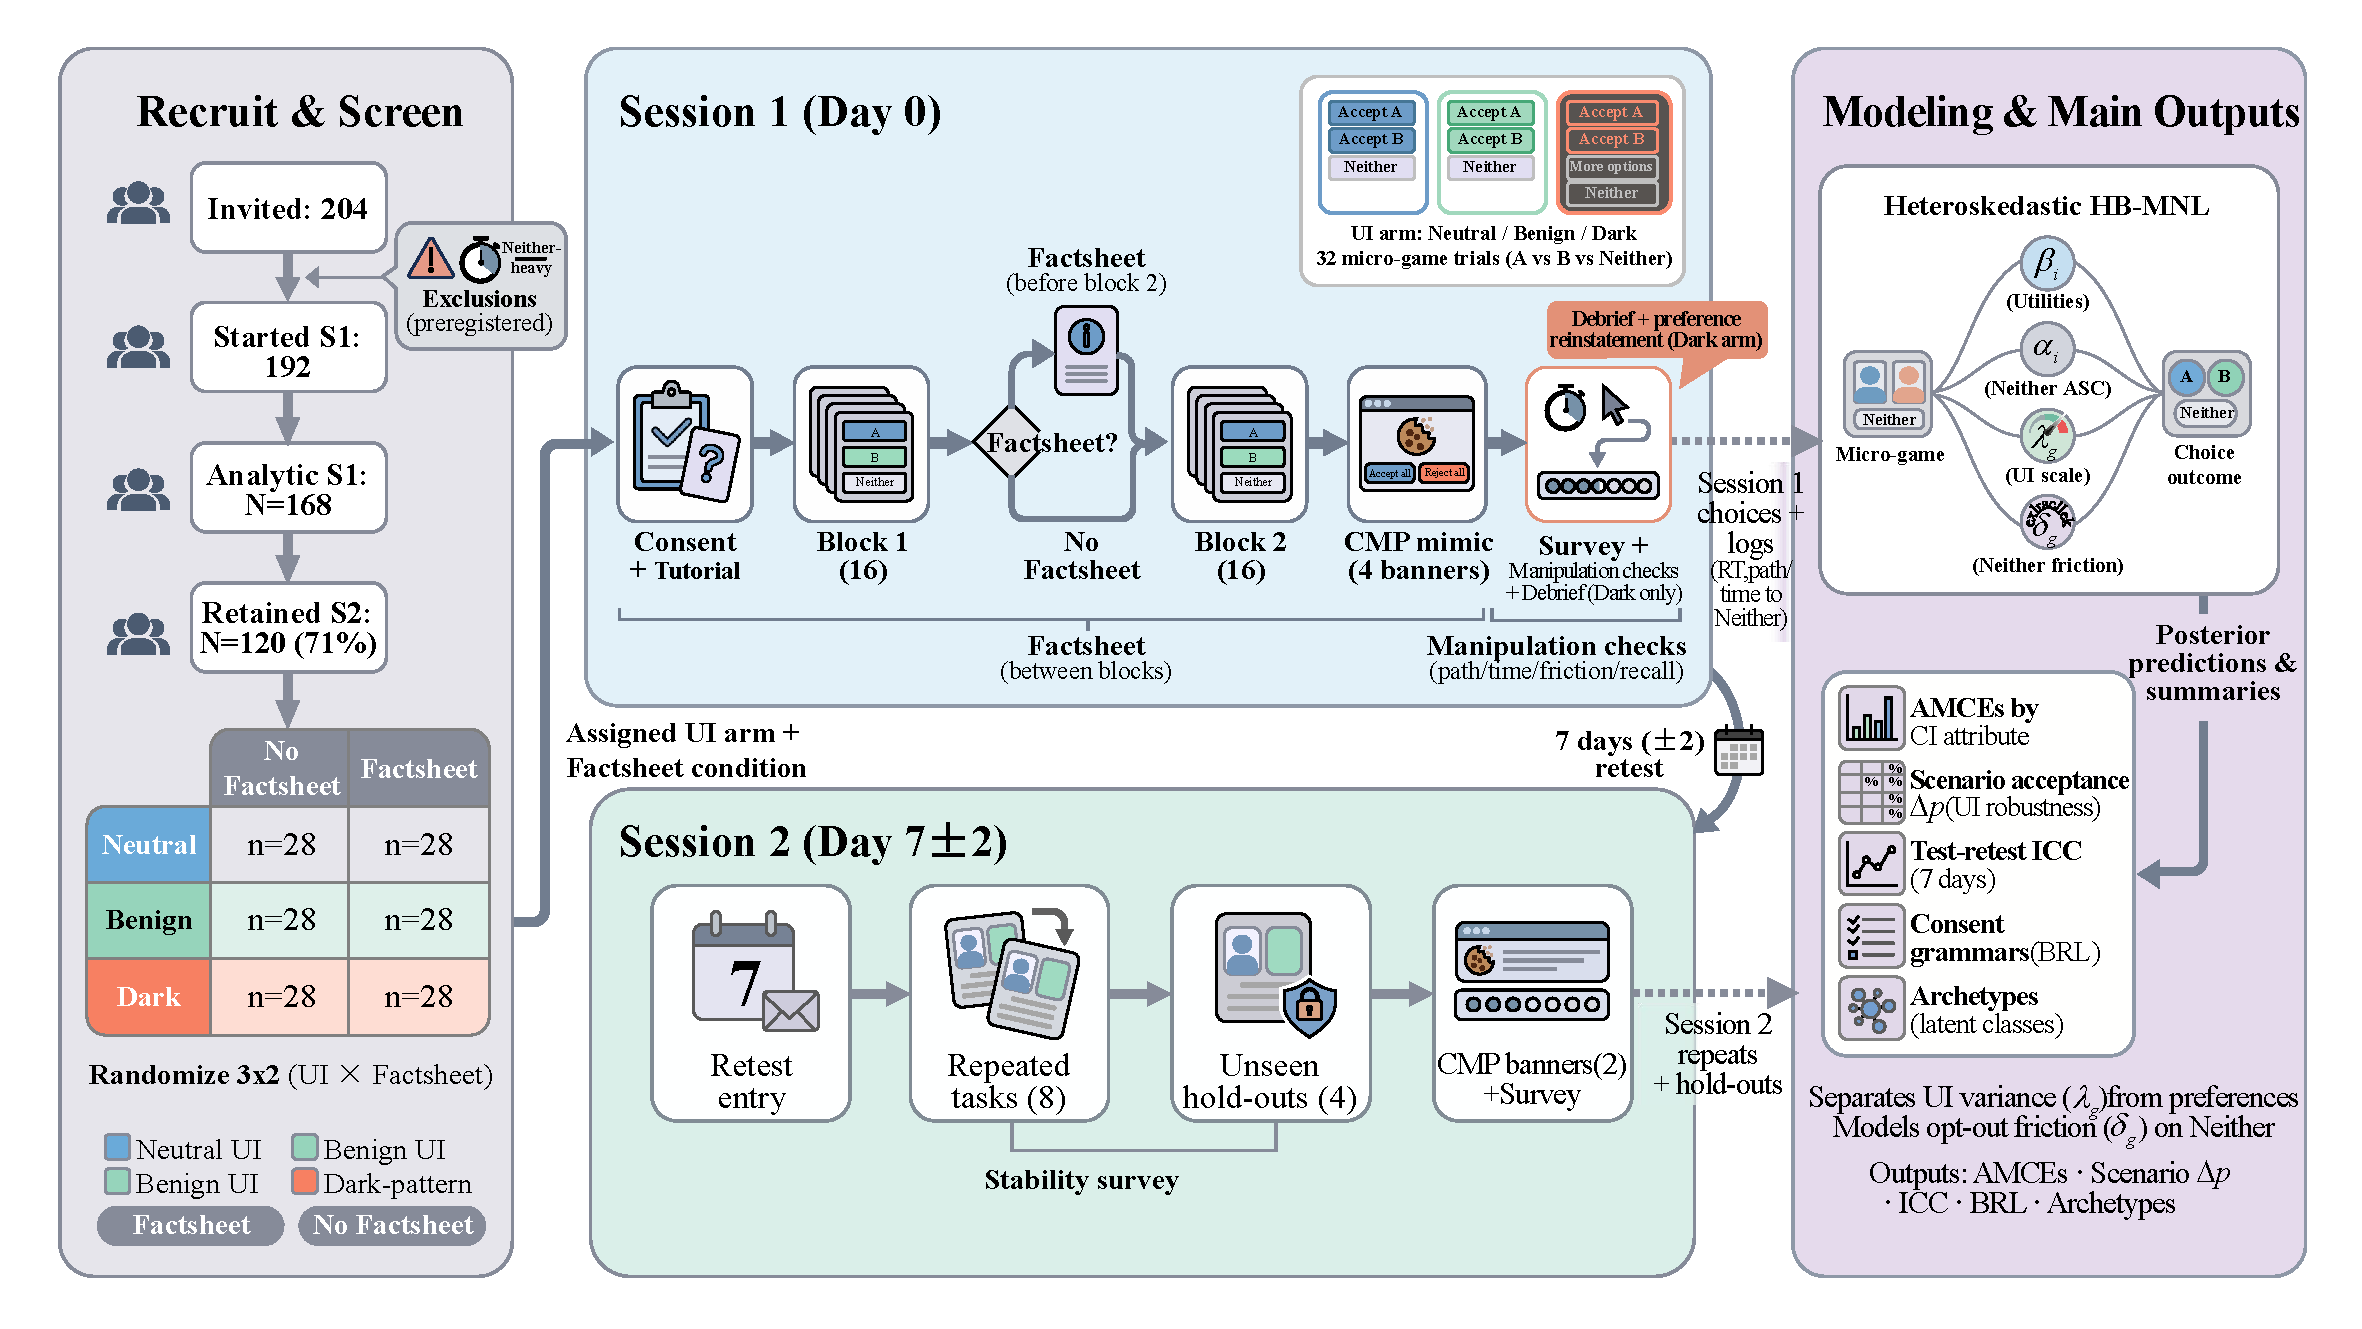
\includegraphics[width=\linewidth]{Figures/Pipeline.pdf}
  \caption{Methodological pipeline: CI-grounded micro-game elicitation, heteroskedastic HB--MNL estimation (separating preference, noise, and opt-out friction), and translation into scenario probabilities, consent grammars, and preference archetypes.}
  \label{fig:pipeline}
\end{figure}

\subsection{Participants and Sampling}
We recruited adult web users via social media who reported English fluency and at least 5 weekly hours of web use, and who had not taken part in pilots. Median completion time was approximately 22 minutes for Session~1 and 12 minutes for Session~2. In total, 204 individuals were invited, 192 consented and started Session~1, and 186 completed all 32 tasks. After predefined exclusions (two comprehension failures, eight extreme speeders, eight with $>$80\% Neither), the Session~1 analytic sample comprised 168 participants, balanced across the $3\times 2$ design (UI $\times$ Factsheet) with 28 per cell. Session~2 retained 120 of 168 (71.4\%). Table~\ref{tab:demographics} summarizes age and gender for the Session~1 analytic sample. Counts are shown to aid reproducibility; percentages are relative to $n{=}168$.
\begin{table}[ht]
  \centering
  \begin{tabular}{lrr @{\hspace{2em}} lrr}
    \multicolumn{3}{c}{\textbf{Age}} & \multicolumn{3}{c}{\textbf{Gender}} \\
    \cmidrule(r){1-3} \cmidrule(l){4-6}
    Category & \textbf{$n$} & \textbf{\%} & Category & \textbf{$n$} & \textbf{\%} \\
    \hline
    18--34 & 70 & 41.7 & Woman & 80 & 47.6 \\
    35--54 & 70 & 41.7 & Man & 80 & 47.6 \\
    55+    & 28 & 16.6 & Non-binary & 8 & 4.8 \\
  \end{tabular}
  \caption{Demographics (Session~1 analytic sample, $n=168$).}
  \label{tab:demographics}
\end{table}

\subsection{Stimuli: Attributes and Levels}
Each profile was formed by orthogonally combining levels with effects coding and a balanced-overlap design to limit cognitive load (Table~\ref{tab:attributes}). No restrictions were imposed on attribute-level combinations; the full factorial serves as a stress test for causal identification~\citep{Hainmueller2014ConjointID}. Comprehension was monitored via attention checks (94.6\% pass rate on an unusual pairing) and stated ANA ($<$7\%; Table~\ref{tab:ana}). As a further robustness check, we re-estimated AMCEs after excluding the four most implausible pairings (e.g., Advertisers~$\times$~Service, Research org~$\times$~Advertising); median absolute AMCE shift was $<0.02$ utils, with no qualitative reversals. Reweighting toward CMP-plausible frequencies likewise leaves AMCEs essentially unchanged (Section~\ref{sec:results}). We used 32 tasks per participant split into two blocks of 16. Of these, 28 were drawn from the D-efficient design and 4 were prespecified \textbf{hold-out tasks} used exclusively for predictive validation (not included in model estimation).

\paragraph{Hold-out task design.}
Four fixed hold-out tasks (positions 8, 16, 24, 32) spanned the attribute space; Session~2 reused two and added two new ones. Multi-class choice accuracy on Session~1 hold-outs was 0.71 (majority baseline 0.52). Full profiles are in Appendix~\ref{app:stimuli}. Because purpose categories can be strategically blurred, P2 (Personalization) and P3 (Advertising) were given distinct, unambiguous descriptions emphasizing whether data is shared externally for ad targeting (verbatim text in Appendix~\ref{app:stimuli}). Both were pre-tested in a pilot ($n=24$; 92\% correct forced-choice classification). In the main study, an attention check testing this distinction yielded a 94.6\% pass rate.

\subsection{User-Interface Arms and Manipulation}
Neutral: symmetric layout with coequal buttons for ``Accept A'', ``Accept B'', and ``Neither/Ask later'', neutral palette, conventional left-to-right order.
Benign variation: non-persuasive layout adjustments (e.g., swapped button order and palette variant) with identical semantics.
Minimal dark-pattern: on the first layer, ``Accept A'' and ``Accept B'' were visible, whereas ``Neither/Ask later'' was placed behind a ``More options'' click. No pre-ticked boxes were used. After the task block, participants received a debrief and could reinstate preferences in a neutral dialog. We instrumented click paths and latency to quantify friction. 
\begin{figure}[h]
  \centering
  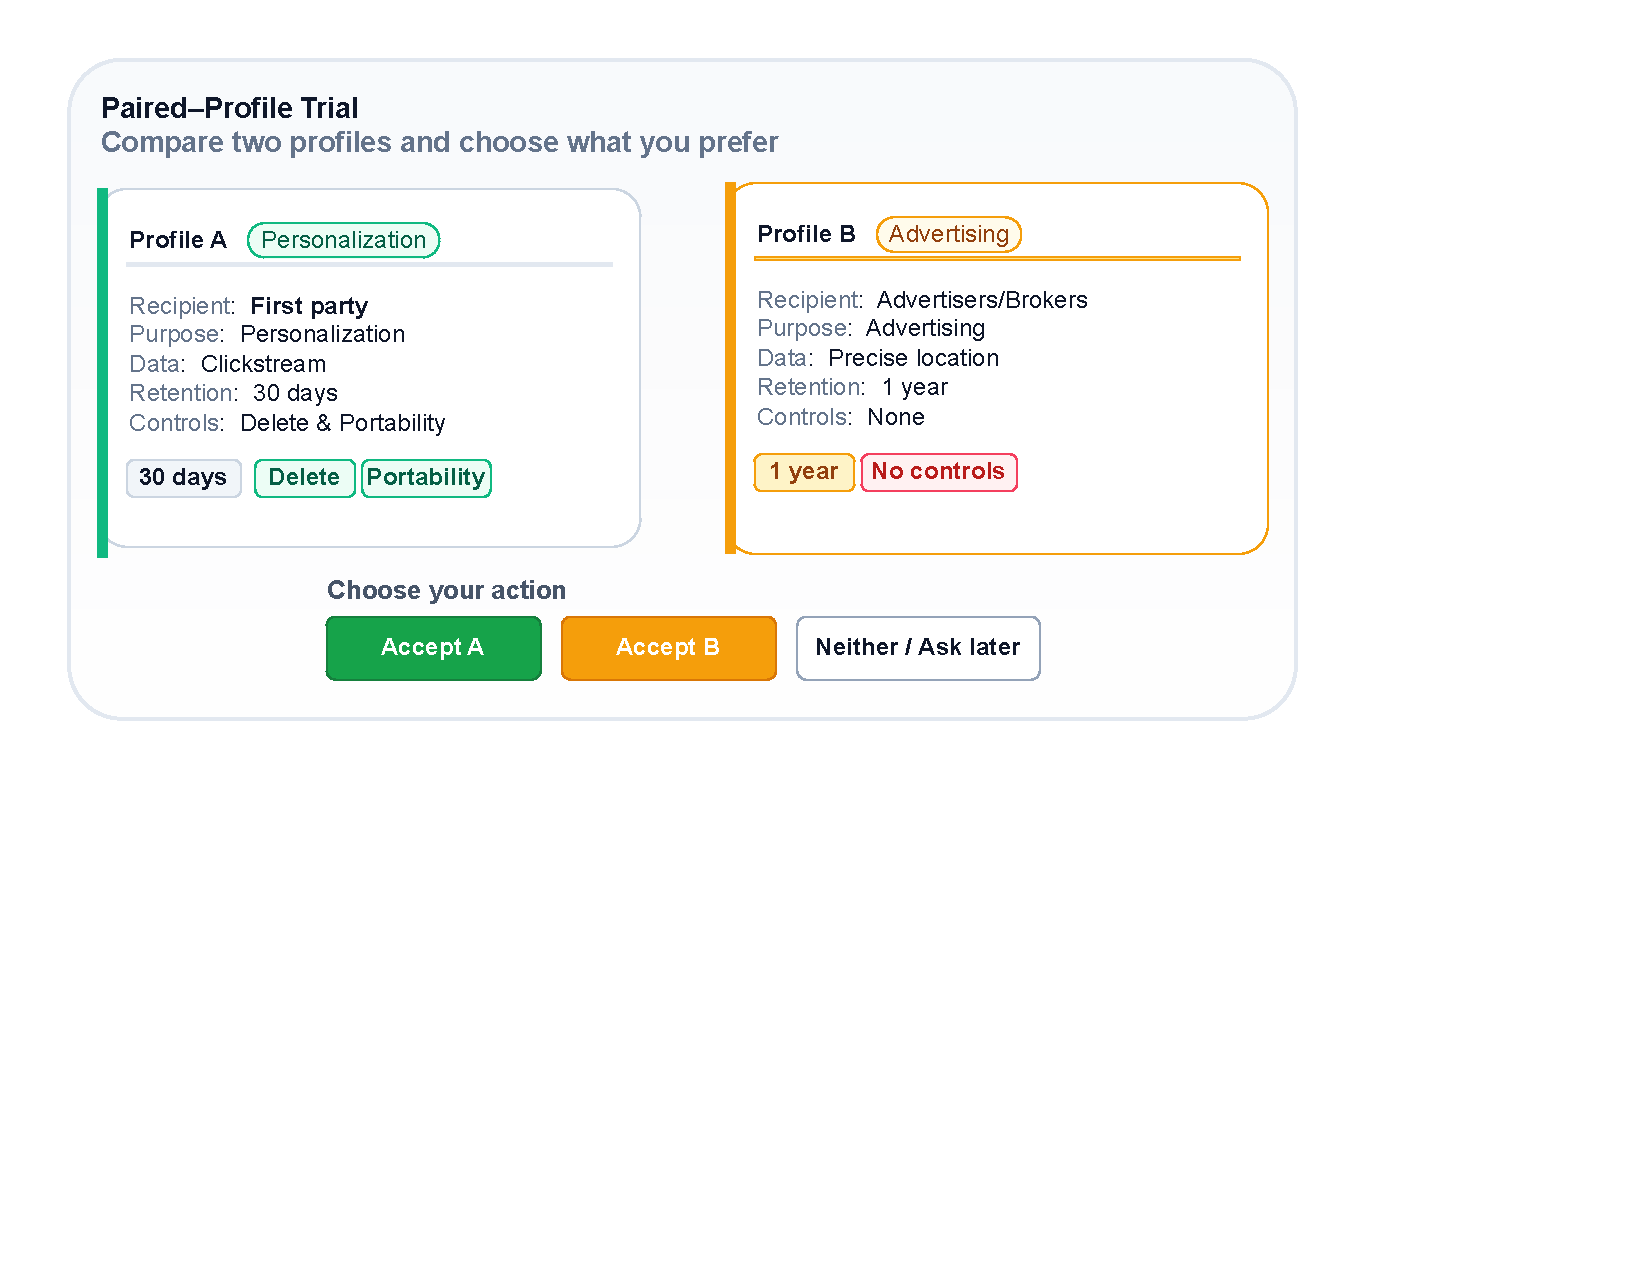
\includegraphics[width=0.85\linewidth]{Figures/ui_new.pdf}
  \caption{Mockup of a paired–profile micro–game trial with Neither/Ask later.}
  \label{fig:attr-card}
\end{figure}
\noindent \textit{CMP mimic parity vs.\ gating.} In the CMP-banner mimic block, Neutral and Benign arms preserved first-layer parity (coequal ``Accept all'' and ``Reject all''). The Dark-pattern arm placed ``Reject all'' behind a More options click (no pre-ticked boxes), mirroring the micro-game manipulation. Full CMP-banner wordings, button layouts, and the Factsheet card (verbatim) are provided in Appendix~\ref{app:stimuli}.



\begin{table}[ht]
    \begin{tabular}{l p{0.6\linewidth}} 
    \textbf{Attribute (CI dimension)} & \textbf{Level label (UI text shown to participants)} \\
    \hline
    \textbf{Recipient} (data recipient) &
    R1: Only this website's servers (first-party) \\
    & R2: This website + its contracted processor (first-party + processor) \\
    & R3: Independent research organization (non-profit) \\
    & R4: Advertising \& data-broker partners (third-party advertisers) \\
    \hline
    \textbf{Purpose / Transmission} &
    P1: Deliver the requested service (functional) \\
    & P2: Personalize content \& recommendations \\
    & P3: Target advertising and measure ads \\
    & P4: Public-interest research (de-identified) \\
    \hline
    \textbf{Data type (attribute)} &
    D1: Basic identifiers (e.g., account ID) \\
    & D2: Clickstream \& page interactions \\
    & D3: Precise location (\(\le 100\) m) \\
    & D4: Sensitive category (e.g., health interest) \\
    \hline
    \textbf{Retention} &
    T1: Session only \\
    & T2: 30 days \\
    & T3: 1 year \\
    & T4: Indefinite \\
    \hline
    \textbf{User controls \& oversight} &
    C1: No additional controls \\
    & C2: Transparency dashboard (view uses) \\
    & C3: Delete \& portability (self-serve) \\
    & C4: Independent privacy audit \& public report \\
  \end{tabular}
  \caption{Attribute taxonomy and operational levels.}
  \label{tab:attributes}
\end{table}

\subsection{Procedure}
\paragraph{Session 1 (Day 0).}
Participants completed consent and screening with a two-item comprehension check (retry allowed), a short tutorial with two warm-up trials, and then 32 paired-profile choice tasks (A vs.\ B vs.\ Neither) in two blocks. Participants assigned to Factsheet viewed a brief neutral information card before Block~2 (explaining ``independent audit'' and ``delete and portability''); those in No Factsheet proceeded directly. At the end of Session~1, participants completed the CMP-banner mimic block (four one-screen banners) and a short survey with manipulation checks. Participants in the dark-pattern arm were debriefed and allowed to reinstate preferences.

\paragraph{Session 2 (Day 7 $\pm$ 2).}
Participants completed a retest consisting of eight repeated tasks and four unseen hold-outs, followed by a brief survey on privacy posture changes. Two CMP mimic banners were used for out-of-session generalization.

\subsection{Manipulation Checks and Instrumentation}
We logged (i) path length to Neither (clicks), (ii) time to Neither (milliseconds), (iii) first-layer attention (recall of decline availability on the first screen), (iv) perceived friction (1--7), and (v) perceived validity (freely given, specific, informed; 1--7). We recorded device class (desktop vs.\ mobile), viewport, region (EU, NA, other), and ad-blocker use.

\subsection{Randomization and Design Generation}
We generated a D-efficient paired-profile design under effects coding with level balance and minimal overlap ($\le 2$ shared attributes per pair). Trial order and left/right placement were independently randomized per participant (cryptographic seeds logged). Five prespecified two-way interactions receive hierarchical-shrinkage priors: R4$\times$T4, P3$\times$D4, P2$\times$D4, R4$\times$C3, and R4$\times$C4, testing whether compounding risks or specific mitigations depart from additivity.

\subsection{Measures}
Primary outcomes: choice (A/B/Neither), response time, hold-out accuracy, and scenario-level acceptance. Secondary: perceived validity, trust, cognitive load, stated ANA, demographics, device, and ad-blocker use (full definitions in Appendix Tables~\ref{tab:variables}--\ref{tab:schema}; analysis plan in Appendix~\ref{subsec:analysis}).

\subsection{Exclusion Criteria}
We applied predefined exclusions: failing both comprehension attempts, median response time $<$1.0 s or $>$50\% of tasks $<$600 ms, failing both attention checks, and choosing ``Neither'' on $>$80\% of tasks. Excluded participants were replaced to maintain cell balance.

\section{Results}
\label{sec:results}

\subsection{Sample, Cells, and Data Quality}
We invited 204 participants; 192 consented and started Session~1; 186 completed all 32 tasks. After predefined exclusions (two comprehension failures, eight extreme speeders, eight with $>$80\% Neither), the Session~1 analytic sample comprised 168, balanced across the $3\times2$ design (UI $\times$ Factsheet) with $n{=}28$ per cell. Session~2 retained 120 of 168 (71.4\%). Median per-task response time in Session~1 was 6{,}685 ms (mean 6{,}716 ms). Choice shares in Session~1 were: Accept~A 0.407, Accept~B 0.404, Neither 0.189. Stated and inferred attribute non-attendance (ANA) were low (Table~\ref{tab:ana}; e.g., Purpose 6.5\% stated / 5.8\% inferred), with no reversals on top-line AMCEs. All Bayesian models converged ($\hat{R}\le 1.01$; effective sample sizes $>\!1000$ per coefficient). Posterior predictive checks indicated good calibration for choice shares and Neither rates.

\subsection{Manipulation Checks and UI-Level Parameters}
The minimal dark-pattern placed Neither/Ask later behind a ``More options'' click on the first layer. Table~\ref{tab:manip} reports Session~1 manipulation checks alongside arm-specific scale ($\lambda$) and the incremental opt-out penalty on Neither ($\delta_g$), compacted into a single table.
\begin{table}[ht]
  \centering
  \resizebox{\linewidth}{!}{%
  \begin{tabular}{l r r r}
    \textbf{Measure} & \textbf{Neutral} & \textbf{Benign} & \textbf{Dark-pattern} \\
    \hline
    Path to ``Neither'' (clicks)         & 1.045 (0.056) & 1.066 (0.065) & \textbf{2.055} (0.120) \\
    Time to ``Neither'' (ms)             & 1651.6 (231.8) & 1655.7 (224.5) & \textbf{2936.3} (248.9) \\
    Perceived friction (1--7)            & 2.403 (0.178) & 2.436 (0.218) & \textbf{3.001} (0.241) \\
    First-layer decline recall (\%)      & 87.6 (5.3) & 85.9 (5.9) & \textbf{39.2} (5.7) \\
    \addlinespace
    Arm scale $\lambda$                  & 1.00 (fixed) & 1.01 [0.93, 1.10] & 0.91 [0.84, 0.99] \\
    Opt-out penalty $\delta_g$ on \Neither{} & 0 (fixed) & $-0.01$ [$-0.05$, $+0.03$] & \textbf{$-0.08$} [$-0.13$, $-0.03$] \\
  \end{tabular}
  }
  \caption{Manipulation checks (Session~1) and UI-level parameters (posterior mean with SD or 95\% HDI). $\delta_g$ is outside $\lambda_g$.}
  \label{tab:manip}
\end{table}

\noindent The dark-pattern arm increased the cost of declining (longer paths and latencies), reduced recall that first-layer refusal was available, and imposed an additional penalty on Neither. To connect friction instrumentation to choice behavior, we decomposed the decline pathway into two observable stages. \emph{Stage~1 (gateway access):} In the Dark arm, 68.2\% [63.4, 72.8] of trials resulted in a click on ``More options'' (the only path to Neither); the remaining 31.8\% never exposed the decline button. In Neutral and Benign arms, Neither was visible on the first layer by design (gateway rate effectively 100\%). \emph{Stage~2 (conditional decline):} Among Dark-arm trials in which participants \emph{did} open ``More options,'' 28.4\% [23.7, 33.5] selected Neither---comparable to the Neutral Neither rate of 26.1\% [22.8, 29.6] (95\% credible intervals from a Bayesian logistic model with participant random intercepts). The difference is small and the intervals overlap, indicating that once the decline option is reached, choosing it is not additionally suppressed. The friction mechanism therefore operates primarily at the \emph{gateway} stage: gating prevents roughly one-third of trials from ever exposing the decline option, and those participants default to accepting one of the two profiles. Among Neither choosers, median time to select Neither was 2{,}891~ms [2{,}714, 3{,}082] in the Dark arm versus 1{,}648~ms [1{,}542, 1{,}761] in Neutral, confirming that the extra click imposes measurable latency even for those who persist. Session-by-session manipulation checks are in Appendix Tables~\ref{tab:manip_session}--\ref{tab:manip_session_2}.

\subsection{RQ-A: Measurement Validity and Stability}
\subsubsection{Individual Consent Boundaries and Hold-Out Prediction}
Table~\ref{tab:amce} reports Average Marginal Component Effects (AMCEs; effects-coded) with 95\% highest-density intervals (HDIs), pooled across UI arms. We show levels 2--4; level~1 is the base: Recipient=First party (R1), Purpose=Service (P1), Data=Basic identifiers (D1), Retention=Session (T1), Controls=None (C1).

\begin{table}[ht]
  \centering
  \begin{tabular}{l l}
    \textbf{Attribute level} & \textbf{AMCE [95\% HDI]} \\
    \hline
    Recipient: R2 Processor                & $-0.014\ [-0.149,\ +0.118]$ \\
    Recipient: R3 Research org             & $+0.316\ [+0.180,\ +0.470]$ \\
    Recipient: R4 Advertisers/Brokers      & $\mathbf{-0.290}\ \mathbf{[-0.450,\ -0.120]}$ \\
    \addlinespace
    Purpose: P2 Personalization            & $-0.116\ [-0.241,\ +0.003]$ \\
    Purpose: P3 Advertising                & $\mathbf{-0.619}\ \mathbf{[-0.798,\ -0.458]}$ \\
    Purpose: P4 Public-interest research   & $\mathbf{+0.185}\ \mathbf{[+0.060,\ +0.310]}$ \\
    \addlinespace
    Data: D2 Clickstream                   & $-0.095\ [-0.235,\ +0.036]$ \\
    Data: D3 Precise location ($\le$100m)  & $\mathbf{-0.607}\ \mathbf{[-0.803,\ -0.445]}$ \\
    Data: D4 Sensitive category            & $\mathbf{-0.512}\ \mathbf{[-0.676,\ -0.352]}$ \\
    \addlinespace
    Retention: T2 30 days                  & $-0.109\ [-0.252,\ +0.021]$ \\
    Retention: T3 1 year                   & $\mathbf{-0.303}\ \mathbf{[-0.459,\ -0.166]}$ \\
    Retention: T4 Indefinite               & $\mathbf{-0.548}\ \mathbf{[-0.710,\ -0.400]}$ \\
    \addlinespace
    Controls: C2 Transparency dashboard    & $+0.082\ [-0.053,\ +0.221]$ \\
    Controls: C3 Delete \& portability     & $\mathbf{+0.428} \mathbf{[+0.284,\ +0.592]}$ \\
    Controls: C4 Independent audit \& report & $\mathbf{+0.324} \mathbf{[+0.212,\ +0.436]}$ \\
  \end{tabular}
  \caption{AMCEs (posterior mean [95\% HDI]) pooled across UI arms. Base levels: R1 First party; P1 Service; D1 Basic identifiers; T1 Session; C1 None. Values shown for levels 2--4.}
  \label{tab:amce}
\end{table}

\noindent Recipient and retention effects are largest in magnitude. Third-party advertisers/data brokers (R4), advertising purpose (P3), precise location (D3), sensitive category (D4), and indefinite retention (T4) reduce acceptance. Concrete protections increase acceptance, with delete/portability (C3) and independent audit (C4) showing the largest positive effects. Figure~\ref{fig:amce_panels} summarizes pooled AMCEs and their practical impact. Multi-class choice accuracy on hold-out tasks was 0.71, exceeding a majority baseline of 0.52. \footnote{The majority baseline (0.52) is computed per hold-out task as the share of the modal choice across participants for that task, then averaged across hold-outs; it is not the global class share.}

\begin{figure}[t]
  \centering
  % Replace with final ABA time‑series plot (vector preferred).
  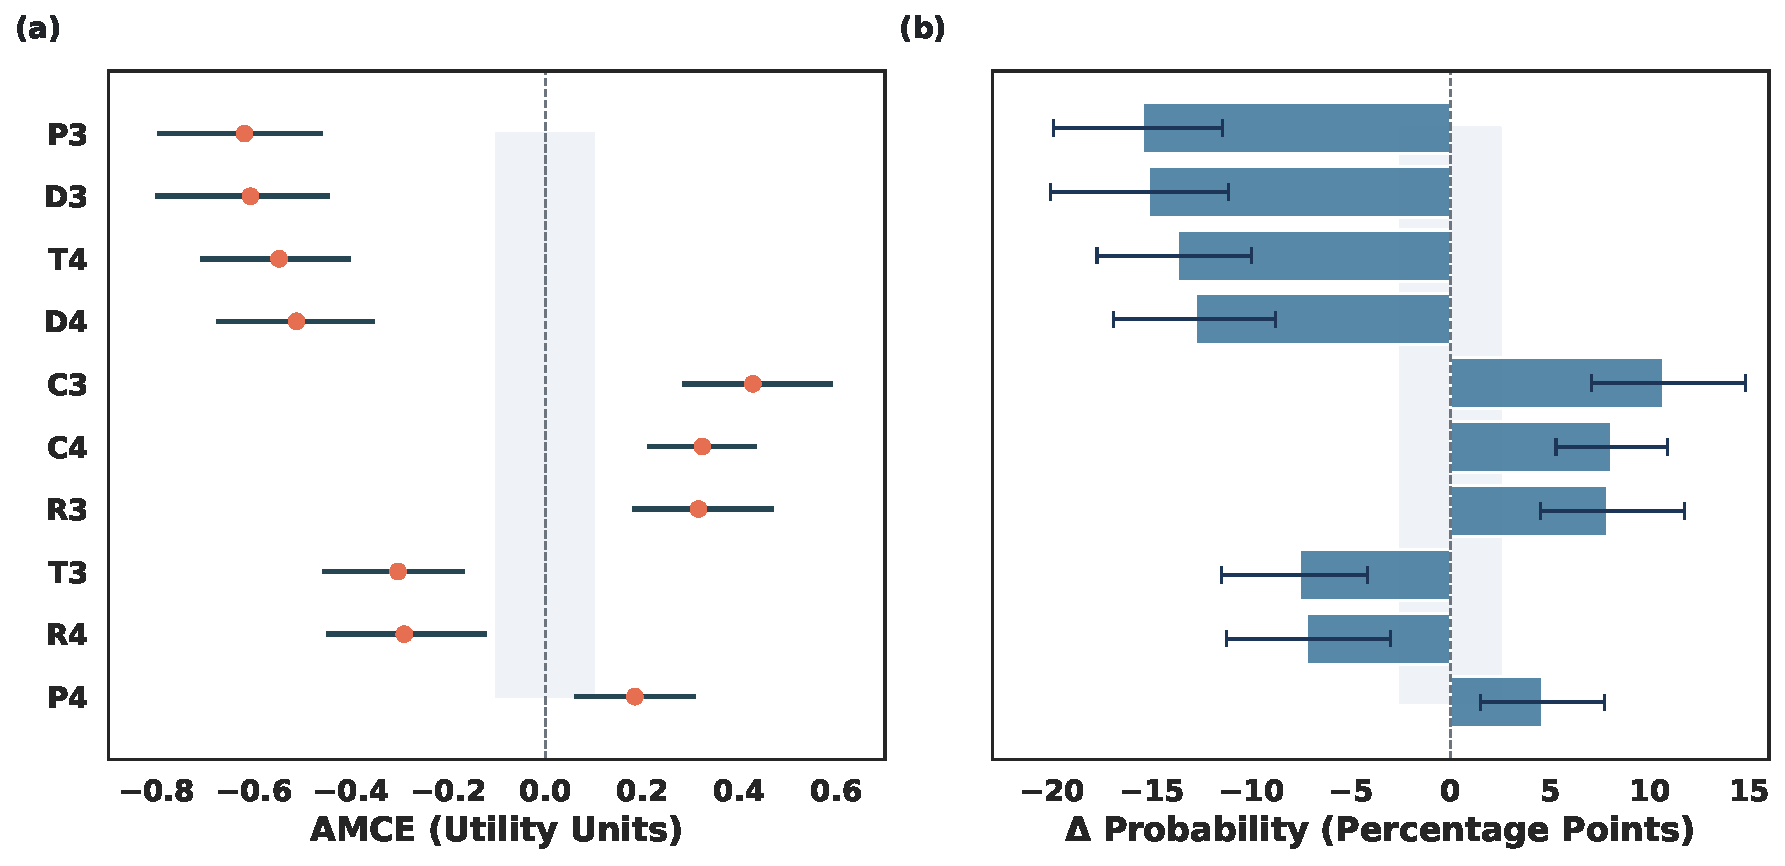
\includegraphics[width=\linewidth]{Figures/fig-amce-panels.pdf}
\caption{Pooled AMCEs and their probability interpretation. Panel (a) shows effects in utility space with 95\% HDIs; panel (b) maps each effect to percentage-point change at baseline $p=0.5$.}
 \label{fig:amce_panels}
\end{figure}
We estimated five CI-motivated interactions with hierarchical shrinkage. The strongest was P3$\times$D4 (Advertising~$\times$~Sensitive: $-1.033$), indicating strong compounding disutility. For Brokers, Independent audit substantially mitigated disutility (R4$\times$C4: $+0.697$; combined offset $\approx$~+1.0 utils), whereas Delete/portability provided only a small incremental offset (R4$\times$C3: $-0.367$; net $\approx$~+0.06). R4$\times$T4 (Brokers~$\times$~Indefinite: $-0.323$) and P2$\times$D4 (near zero: $-0.047$) complete the set. In policy-equivalent terms, Independent audit is roughly comparable to shortening retention by one step; Delete/portability exceeds one step; offsetting a move to Brokers typically requires a bundle of protections plus shorter retention.

\paragraph{Purpose-label sensitivity.}
The near-zero P2$\times$D4 interaction ($-0.047$) versus the large P3$\times$D4 ($-1.033$) implies that the purpose label alone can shift consent boundaries substantially. Table~\ref{tab:purpose_label} isolates this effect by computing posterior-predictive acceptance for a fixed profile under the two purpose labels.

\begin{table}[ht]
  \centering
  \begin{tabular}{l c}
    \textbf{Purpose label} & \textbf{Predicted acceptance [\%] [95\% HDI]} \\
    \hline
    P3: Advertising       & 14 [11, 18] \\
    P2: Personalization   & 31 [27, 36] \\
    \addlinespace
    Difference (P2$-$P3)  & \textbf{+17} [+13, +22] \\
  \end{tabular}
  \caption{Purpose-label sensitivity for a fixed profile (Brokers, Sensitive, 1~year, no controls). Relabeling the purpose from Advertising to Personalization raises predicted acceptance by 17\,pp [95\% HDI], holding all other attributes constant.}
  \label{tab:purpose_label}
\end{table}

\subsubsection{Stability Over One Week (Test--Retest)}
Test--retest agreement over 7 days was moderate. Task-level ICC (on logit-transformed posterior-mean predicted acceptance) was 0.68 [0.61, 0.74]. Blockwise utility composites (summing posterior-mean $\hat{\beta}_{i,k}$ within each attribute block) yielded ICCs from 0.55 (Purpose) to 0.72 (Retention). Rank stability: median Spearman $\rho\approx 0.62$.

\subsubsection{Information Effects (Factsheet Intervention)}
Table~\ref{tab:factsheet} summarizes Factsheet effects. Effects are small-to-moderate: the Factsheet slightly increases the value of Independent audit (C4) and the Neither constant ($\alpha$), while modestly decreasing acceptance for Indefinite retention. Arm~$\times$~Factsheet interactions are negligible, indicating that information effects are independent of the UI manipulation.

\begin{table}[ht]
  \centering
  \resizebox{\linewidth}{!}{%
  \begin{tabular}{l r}
    \textbf{Estimand} & \textbf{$\Delta$ (Factsheet)} \\
    \hline
    Controls: Delete \& portability (C3) & $+0.04\ [ -0.01,\ +0.09 ]$ \\
    Controls: Independent audit (C4)     & $\mathbf{+0.06}\ \mathbf{[+0.01,\ +0.11]}$ \\
    Retention: Indefinite (T4)           & $\mathbf{-0.05}\ \mathbf{[-0.10,\ -0.00]}$ \\
    Purpose: Advertising (P3)            & $-0.04\ [-0.09,\ +0.01]$ \\
    \addlinespace
    \Neither{} constant $\Delta\alpha$   & $\mathbf{+0.05}\ \mathbf{[+0.01,\ +0.09]}$ \\
    \addlinespace
    Scenario S1 (Service, identifiers, 30d, none)        & $-0.5$\% $[-1.8,\ +0.7]$ \\
    Scenario S2 (Personalization, clickstream, 1y, dash) & $-1.2$\% $[-2.8,\ +0.3]$ \\
    Scenario S3 (Brokers, sensitive, indefinite, none)   & $-0.8$\% $[-2.6,\ +1.0]$ \\
    \addlinespace
    Arm $\times$ Factsheet interactions (max $|\Delta|$) & $< 0.02$ utils (all HDIs overlap 0) \\
  \end{tabular}
  }
  \caption{Factsheet effects: Factsheet minus No-Factsheet (posterior mean [95\% HDI]). Positive means more acceptable.}
  \label{tab:factsheet}
\end{table}

\subsection{RQ-B: UI Mechanism---Robustness, Scale, and Opt-Out Friction}
Table~\ref{tab:manip} reports arm-specific scale and opt-out parameters alongside manipulation checks. The Benign arm is indistinguishable from Neutral on all measures; the Dark arm shows lower scale ($\lambda \approx 0.91$) and a credible opt-out penalty ($\delta \approx -0.08$). We report scenario-level acceptance differences as the primary UI comparison (Table~\ref{tab:scenarios}): the Dark arm raises acceptance by +3--7\,pp, with the largest increase for the ad-tech profile. To avoid scale--taste confounding, we do not interpret cross-arm coefficients; all comparisons are calibrated scenario probabilities. Figure~\ref{fig:ui_panels} synthesizes these effects.


\begin{figure}[t]
  \centering
  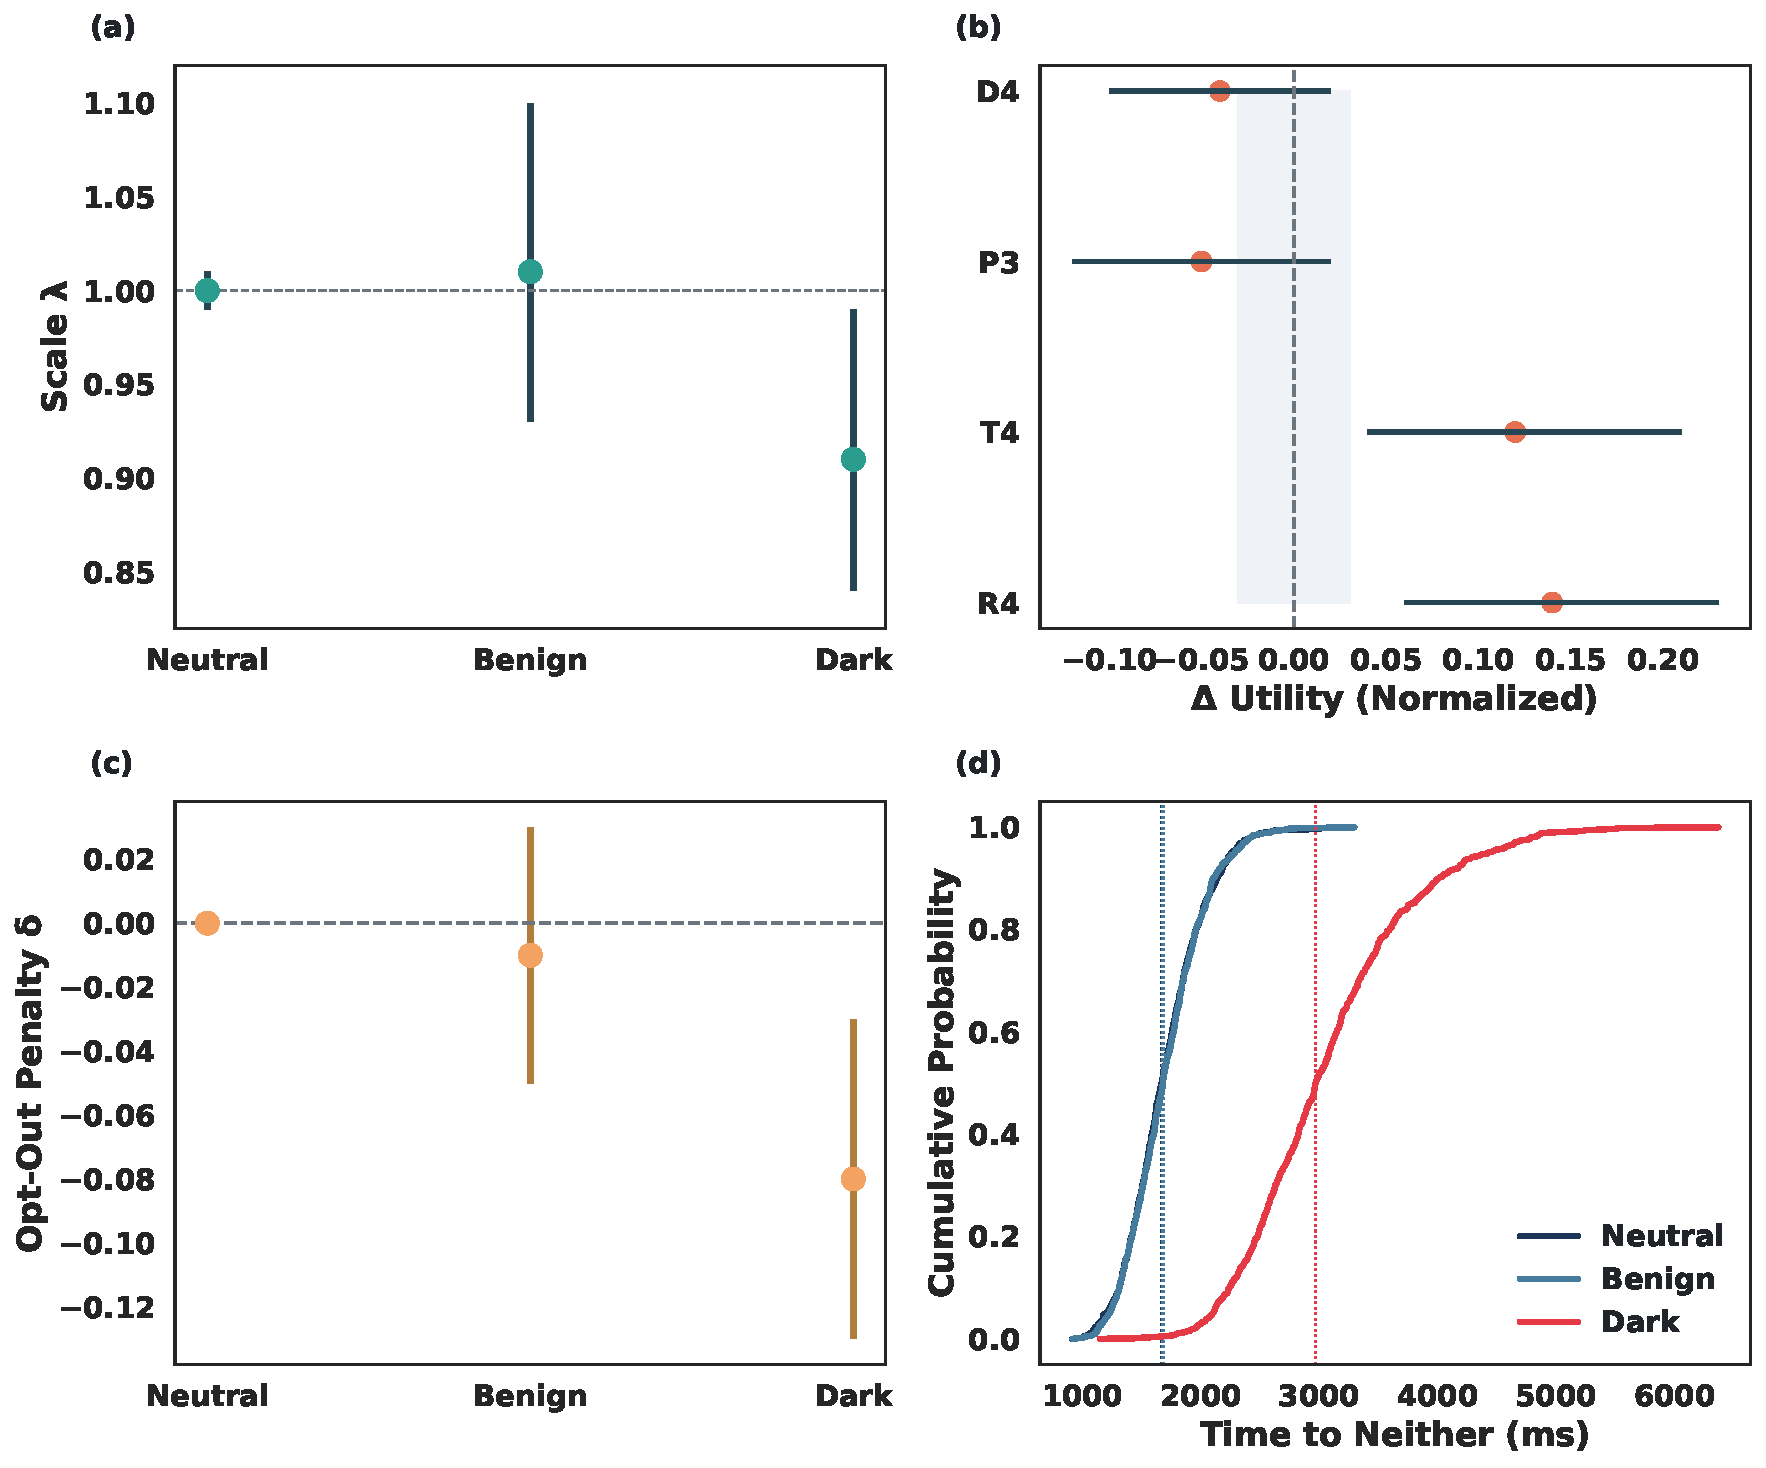
\includegraphics[width=\linewidth]{Figures/fig-ui-panels.pdf}
  \caption{UI robustness and opt-out friction. Panel~(a) arm-specific scale; 
(b) normalized coefficients (no inference; UI comparisons are made at scenario level); 
(c) incremental opt-out penalty on \Neither{}; (d) accumulated delay to opt out by arm.}
  \label{fig:ui_panels}
\end{figure}


\begin{table}[ht]
  \centering
  \resizebox{\linewidth}{!}{%
  \begin{tabular}{@{} l c c c @{}}
    \textbf{Scenario} & \textbf{Neutral} & \textbf{Benign ($\Delta$)} & \textbf{Dark ($\Delta$)} \\
    \hline
    S1: Service, identifiers, 30d, no controls & 63 [59, 67] & 64 (+1) [60, 68] & 66 (+3) [62, 70] \\
    S2: Personalization, clickstream, 1y, dashboard & 52 [48, 56] & 53 (+1) [49, 57] & 56 (+4) [52, 60] \\
    S3: Brokers, sensitive, indefinite, no controls & 24 [21, 28] & 25 (+1) [22, 29] & \textbf{31 (+7)} [27, 35] \\
  \end{tabular}
  }
  \caption{Scenario acceptance (\%; posterior mean [95\% HDI]). $\Delta$ columns show percentage-point change vs.\ Neutral.}
  \label{tab:scenarios}
\end{table}

\paragraph{Substitution patterns under friction.}
To characterize where suppressed Neither choices migrate, we identified \emph{high-abstention trials}: task--participant pairs in which the posterior-mean predicted Neither probability under the Neutral model (i.e., setting $\delta_g{=}0$ and $\lambda_g{=}1$ while retaining participant-specific $\beta_i$ and $\alpha_i$) exceeded 0.30. This threshold isolates trials where abstention was a plausible choice under friction-free conditions; results are qualitatively stable under thresholds of 0.25 and 0.35. Within this subset, we computed arm-specific choice shares and bootstrapped 95\% intervals (10{,}000 resamples, clustered by participant; we use bootstrap rather than posterior intervals here because this analysis operates on observed choice shares, not on the HB--MNL posterior). In the Dark arm, the Neither share dropped from 0.34 [0.30, 0.38] (Neutral) to 0.22 [0.18, 0.26], a displacement of 0.12 [0.07, 0.17]. The displaced share was redistributed unevenly: the profile with higher posterior-mean predicted utility absorbed 0.08 [0.05, 0.12] of the shift, versus 0.04 [0.02, 0.07] for the lower-utility profile (ratio $\approx$~2.1:1 [1.4, 3.2]). This asymmetric substitution indicates that friction selectively pushes would-be abstainers toward the more attractive profile rather than inflating acceptance uniformly, consistent with a threshold mechanism in which gating raises the cost of declining without altering the relative attractiveness of A versus B.

Reweighting profiles to CMP-mimic frequencies left AMCEs essentially unchanged (median shift $<0.03$). In the CMP-banner mimic block, accept rates were Neutral 56.6\%, Benign 54.8\%, Dark 62.0\% (Dark--Neutral $\approx$ +5.4\,pp). Individual Neither propensity aligned with CMP Reject-all ($\rho=0.49$; partial $\rho\approx 0.40$ controlling for profile attractiveness).


A logistic classifier predicting the binary CMP mimic outcome from micro-game-derived acceptance probabilities achieved AUC~$= 0.72$ [0.67, 0.77]; adding Neither propensity ($\alpha_i$) raised AUC to 0.76 [0.71, 0.80] with reasonable calibration (ECE~$= 0.041$). The moderate AUC is expected given the different cognitive demands of a one-screen banner versus a deliberative micro-game; we interpret the link as evidence that micro-game boundaries capture a meaningful component of real-banner behavior (Figure~\ref{fig:cmp_panels}).

\begin{figure}[t]
  \centering
  % Replace with final ABA time‑series plot (vector preferred).
  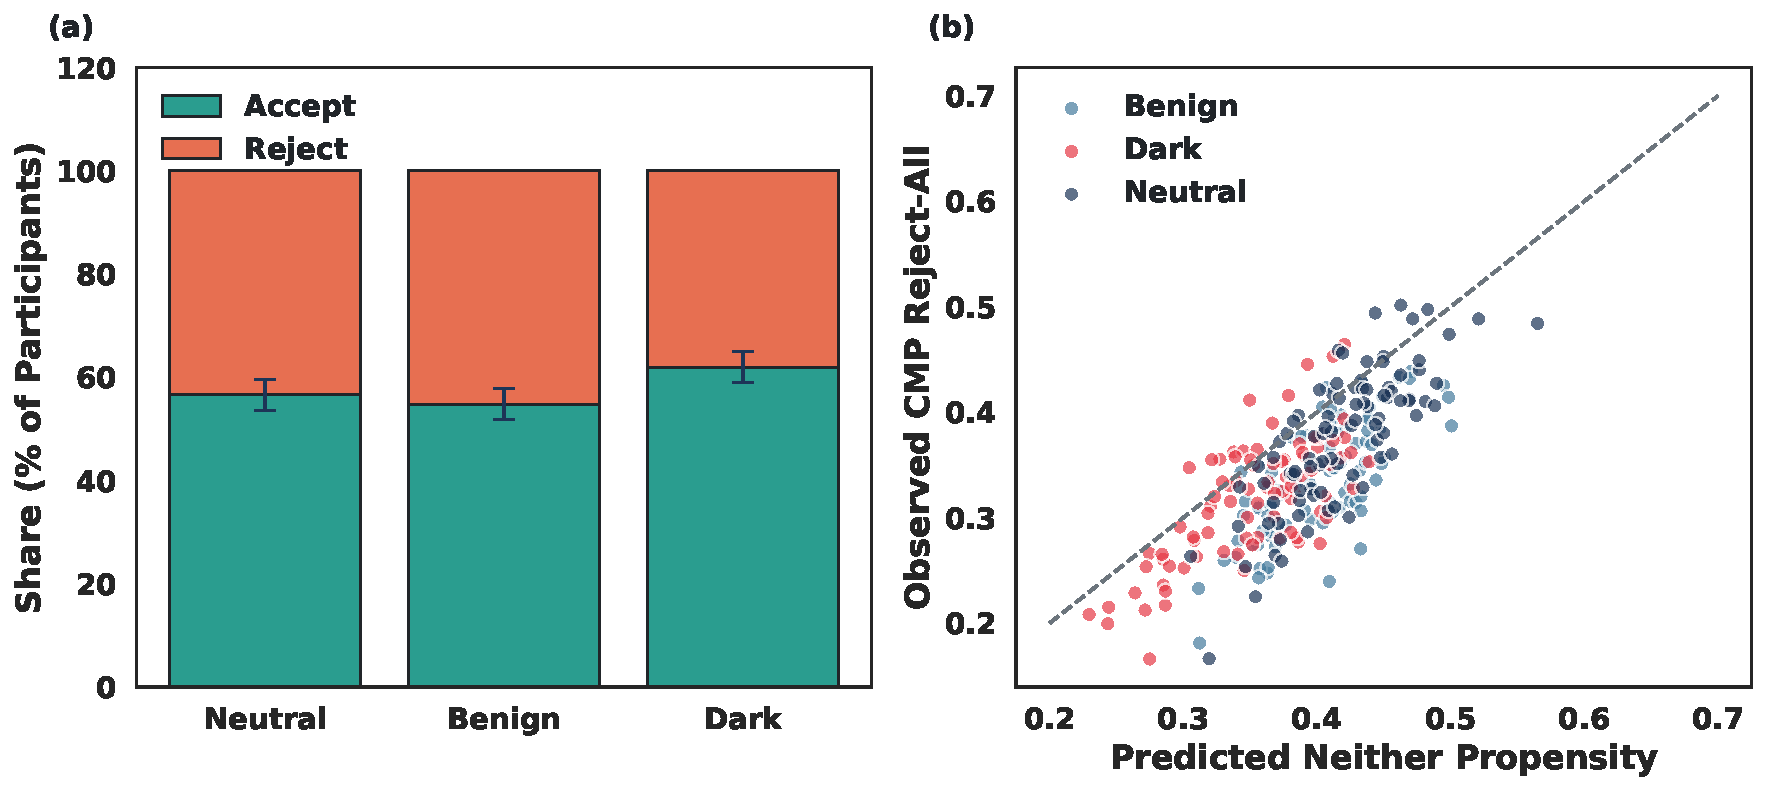
\includegraphics[width=\linewidth]{Figures/fig-cmp-panels.pdf}
  \caption{CMP mimic outcomes and construct alignment. The Dark arm increases accept rates (panel~a). Participant-level Neither propensity aligns with CMP Reject-all (panel~b).}
  \label{fig:cmp_panels}
\end{figure}

\subsection{RQ-C: Translation and Deployment}
\subsubsection{Interpretable Consent Grammars (Bayesian Rule Lists)}
Rule lists approximated HB predictions on hold-outs with high fidelity and modest complexity (AUC \(\approx 0.83{-}0.86\), median length 4). Stability across sessions was reasonable by rule overlap (Jaccard \(\approx 0.74\)).

\begin{table}[h]
  \centering
  \begin{tabular}{l l l l}
    \textbf{Arm} & \textbf{AUC} & \textbf{Accuracy} & \textbf{Rule length} \\
    \hline
    Neutral       & 0.86 [0.82, 0.89] & 0.80 [0.76, 0.84] & 4 [3, 5] \\
    Benign        & 0.85 [0.82, 0.88] & 0.79 [0.75, 0.83] & 4 [3, 5] \\
    Dark-pattern  & 0.83 [0.79, 0.86] & 0.78 [0.73, 0.81] & 4 [3, 5] \\
  \end{tabular}
  \caption{Grammar fidelity and complexity (median [IQR]).}
  \label{tab:brl}
\end{table}

\noindent \textbf{Example rule (Neutral arm).}
\begin{quote}\small
IF Recipient=Advertisers/Brokers AND Retention$\ge$1~year $\Rightarrow$ DECLINE;\\
ELSE IF Data=Sensitive AND Purpose=Advertising $\Rightarrow$ DECLINE;\\
ELSE IF Controls$\in$\{Independent Audit, Delete \& Portability\} AND Retention$\le$30~days $\Rightarrow$ ACCEPT;\\
ELSE $\Rightarrow$ NEITHER.
\end{quote}

\subsubsection{Preference Archetypes, Stability, and Cold-Start}
We estimated a finite mixture of multinomial logit models on scale-normalized individual utilities ($\hat{\beta}_i / \hat{\lambda}_{g(i)}$), with $K \in \{2,\ldots,6\}$ classes and symmetric Dirichlet(1) mixing weights. Each class has its own mean utility vector; we selected $K{=}4$ by WAIC. Table~\ref{tab:archetypes} summarizes their defining characteristics and scenario-level acceptance (posterior-mean class-conditional predictions with 95\% HDIs). Class~1 (\emph{First-party pragmatists}, 34\%) accepts most first-party functional flows but declines third-party sharing; retention is a secondary concern. Class~2 (\emph{Anti-ad-tech absolutists}, 22\%) exhibits strong across-the-board rejection of advertising and broker recipients regardless of controls; Neither rates are the highest of any class. Class~3 (\emph{Governance-trusting sharers}, 26\%) tolerates broader sharing when independent audit or delete/portability is present; the R4$\times$C4 interaction is especially pronounced. Class~4 (\emph{Data minimizers}, 18\%) is driven primarily by retention and data-type sensitivity, with indefinite retention and precise location as dominant rejection triggers. Class stability was high: bootstrap ARI~$\approx$~0.78; split-half NMI~$\approx$~0.72. Cold-start: a 3-question policy assigned classes with 0.71 accuracy; 5 questions reached 0.78 on Session~2; performance was similar on the CMP mimic banners.

\begin{table}[h]
  \centering
  \resizebox{\linewidth}{!}{%
  \begin{tabular}{@{} l c l c c @{}}
    \textbf{Archetype} & \textbf{Share} & \textbf{Defining features} & \textbf{S1 accept [\%]}  & \textbf{S3 accept [\%]} \\
    \hline
    1: First-party pragmatists & 34\% & Low R4/P3 disutility; moderate retention sensitivity & 78 [73, 83] & 18 [14, 23] \\
    2: Anti-ad-tech absolutists & 22\% & Strong R4 + P3 penalty; high Neither rate & 51 [45, 57] & 8 [5, 12] \\
    3: Governance-trusting sharers & 26\% & Large C4/C3 gains; R4$\times$C4 mitigates brokers & 70 [64, 76] & 34 [28, 40] \\
    4: Data minimizers & 18\% & Retention + data-type dominant; location/sensitive $\gg$ purpose & 58 [51, 65] & 12 [8, 17] \\
  \end{tabular}
  }
  \caption{Preference archetypes from scale-normalized latent-class mixture ($K{=}4$ by WAIC). Acceptance rates are posterior means [95\% HDI]. S1 = Service, identifiers, 30d, no controls; S3 = Brokers, sensitive, indefinite, no controls.}
  \label{tab:archetypes}
\end{table}

\subsubsection{Perceived Validity and Alignment with Decisions}
Perceived validity (freely given, specific, informed; 1--7) increased with concrete protections and decreased for advertising recipients, advertising purpose, and indefinite retention. Validity positively predicted acceptance and negatively predicted Neither.

\begin{table}[h]
  \centering
  \begin{tabular}{l l}
    \textbf{Predictor} & \textbf{Effect on validity} \\
    \hline
    Recipient: Advertisers/Brokers & $-0.48\ [-0.60,\ -0.35]$ \\
    Retention: Indefinite & $-0.37\ [-0.48,\ -0.25]$ \\
    Purpose: Advertising & $-0.29\ [-0.40,\ -0.18]$ \\
    Controls: Independent audit & $+0.31\ [+0.20,\ +0.41]$ \\
    Controls: Delete \& portability & $+0.22\ [+0.12,\ +0.32]$ \\
    \addlinespace
    Validity $\rightarrow$ Acceptance (logit slope) & $+0.44\ [+0.33,\ +0.55]$ \\
    Validity $\rightarrow$ ``Neither'' (logit slope) & $-0.27\ [-0.38,\ -0.16]$ \\
  \end{tabular}
  \caption{Perceived validity and behavioral alignment (standardized effects: posterior mean [95\% HDI]).}
  \label{tab:validity}
\end{table}

\subsection{Ecological Validity Checks}
\label{subsec:ecological}
Response time decreased sharply during the first four trials (8{,}412~ms $\to$ 6{,}205~ms) and then stabilized for the remainder of Session~1 (post-warm-up slope indistinguishable from zero: $-8$~ms/trial [$-24$, $+9$]). Neither rates and acceptance rates showed a complementary warm-up effect (Neither slightly elevated in trials 1--4 at 0.22 vs.\ 0.18 thereafter) but no monotonic drift post-warm-up (Neither OR~$= 1.002$ per trial [0.996, 1.008]; Acceptance OR~$= 0.999$ [0.994, 1.004]). These patterns are consistent with task familiarization rather than fatigue or learning. We retain all 32 trials for estimation; hold-out accuracy (0.71) provides a further internal validity check.

\subsection{Subgroup Heterogeneity and Fairness}
\label{subsec:subgroup}
Table~\ref{tab:subgroup} reports the largest posterior deviations from pooled AMCEs across age, gender, device, region, and ad-blocker splits. All deviations are small relative to main effects, with credible intervals overlapping zero in every case; no qualitative reversals were observed.


\begin{table}[ht]
  \centering
  \resizebox{\linewidth}{!}{%
  \begin{tabular}{l l r r}
    \textbf{Subgroup} & \textbf{Attribute level} & \textbf{$\Delta$ from pooled} & \textbf{95\% HDI} \\
    \hline
    Age 55+ & T4 Indefinite & $-0.09$ & [$-0.18$, $+0.01$] \\
    Age 55+ & C4 Independent audit & $+0.07$ & [$-0.02$, $+0.16$] \\
    Ad-blocker users & R4 Advertisers/Brokers & $-0.06$ & [$-0.14$, $+0.03$] \\
    EU (vs.\ NA) & R4 Advertisers/Brokers & $-0.05$ & [$-0.12$, $+0.02$] \\
    Mobile (vs.\ desktop) & Neither constant $\alpha$ & $-0.04$ & [$-0.10$, $+0.02$] \\
    Women (vs.\ men) & P3 Advertising & $-0.03$ & [$-0.11$, $+0.05$] \\
  \end{tabular}
  }
  \caption{Largest subgroup deviations from pooled AMCEs (posterior mean [95\% HDI]). All intervals overlap zero; no qualitative reversals were observed.}
  \label{tab:subgroup}
\end{table}


Grammar AUC ranged from 0.82 to 0.87 across subgroups (max gap 0.04); archetype cold-start accuracy ranged from 0.68 to 0.74 (max gap 0.05). These splits are reported \emph{solely for fairness auditing}; we explicitly advise against using demographic attributes as inputs to personalization or archetype assignment.

\subsection{Additional Results}
A mixture extension including excluded high-abstention participants (prevalence 4.7\%) left core estimands essentially unchanged (AMCE shifts $<\!0.03$; $\delta_{\text{Dark}}$ and $\lambda_{\text{Dark}}$ stable). No qualitative reversals emerged by region or device. Sensitivity analyses (multinomial probit, nested logit, GMNL, ANA re-estimation, CMP-weighted profiles) appear in the Appendix.
%========================================
\section{Discussion}
\label{sec:discussion}

\paragraph{Consent boundaries and CI alignment.}
Recipients and retention are the dominant drivers of acceptance, while concrete protections---especially Delete/portability and Independent audit---deliver the largest positive shifts (Table~\ref{tab:amce}). This pattern is consistent with Contextual Integrity, which emphasizes that actors and transmission principles govern the acceptability of information flows~\citep{Nissenbaum2004ContextualIntegrity,MartinNissenbaum2016MeasuringPrivacy}. It also aligns with empirical evidence that tangible safeguards (e.g., retention limits, deletion/portability, oversight) increase willingness to share sensitive data \citep{Gupta2023ConsumerViewsJAMA}. In policy-equivalent terms, we estimate that Independent audit is roughly comparable to shortening retention by one step (e.g., 1y$\to$30d), with Delete/portability slightly larger; this is directionally compatible with regulatory guidance that emphasizes valid, informed consent and meaningful post‑consent controls.

Two interactions are especially actionable. Advertising paired with Sensitive data carries strong compounding disutility, consistent with CI's prediction that purpose and attribute jointly shape norms~\citep{Nissenbaum2004ContextualIntegrity,MartinNissenbaum2016MeasuringPrivacy}. For Brokers, Independent audit offsets a large share of the disutility (main $+$ interaction $\approx$ +1.0 utils), whereas Delete/portability provides only a small incremental offset, suggesting that oversight and accountability are perceived as qualitatively different from post-hoc data operations. The P3$\times$D4 asymmetry exposes a vulnerability to \emph{purpose laundering}: for a matched Brokers profile (Sensitive, 1~year, no controls), relabeling the purpose from Advertising to Personalization raises predicted acceptance from 14\% to 31\%---a 17-percentage-point gap attributable solely to the purpose label. Our consent grammars can detect such boundary violations, and Independent audit provides a mechanism to verify that stated purposes match actual practice.

\paragraph{UI mechanism: friction, noise, and preference separation.}
The minimal dark pattern both reduces scale and imposes a selective opt-out penalty, raising scenario-level acceptance by 3--7\,pp for ad-tech cases---consistent with reports that first-layer asymmetries materially raise acceptance without improving understanding~\citep{Nouwens2020CHI,Habib2022CHI,Bielova2024USENIX,Berens2024CoSe} and with regulatory guidance identifying selective friction as a deceptive practice~\citep{EDPB2023DarkPatterns,ICO_CMA_2023_HarmfulDesign}. Preferences are robust across Neutral and Benign arms ($|\Delta| \le 1$\,pp), and reweighting to CMP-style profile frequencies leaves AMCEs unchanged. Neither propensity aligns with CMP Reject-all ($\rho = 0.49$; AUC~$= 0.76$), indicating that the instrument captures a meaningful component of real-world consent decisions. Our UI claims are scoped to one friction mechanism and one benign variation; they do not extend to the full dark-pattern design space. For future stated-choice work, we recommend scale-normalized arm contrasts with an explicit opt-out mechanism~\citep{Swait1993SL,Fiebig2010GMNL} and profile-distribution sensitivity analyses~\citep{de2022improving}.

\paragraph{Consent as socio-technical governance.}
Consent on the Web is a socio-technical arrangement in which platforms, CMPs, and advertisers jointly shape the conditions under which users exercise meaningful choice. CMP audits~\citep{Nouwens2020CHI,Matte2020DoCookieBannersRespect,Bielova2024USENIX} show that the burden falls almost entirely on individuals; our findings confirm that a single extra click on the refusal path raises acceptance by 3--7\,pp while preferences remain unchanged. The micro-game redistributes this burden. Consent grammars make boundaries \emph{inspectable} and \emph{contestable}: users can read, edit, and override rules, and the decision log provides a trail for review. For regulators, the friction diagnostic ($\delta_g$) operationalizes the ``freely given'' criterion; grammar-based boundary comparison detects purpose laundering; and archetypes serve as \emph{population-level baselines} against which a CMP's consent rates can be benchmarked. This positions the toolkit as a \emph{governance instrument} rather than an optimization tool. For implementers, first-layer parity and the removal of selective opt-out friction are essential; Independent audit and Delete/portability are the highest-leverage protections. The micro-game is a \emph{deliberative measurement instrument}---akin to a privacy preference center---whose moderate alignment with CMP mimic behavior (AUC~$\approx$~0.76; $\rho = 0.49$) confirms that it captures a meaningful component of real-world consent decisions.

\paragraph{Deployment, risks, and misuse.}
Deployment requires six non-negotiable guardrails: (1)~first-layer parity, (2)~no nudging, (3)~user agency (every decision overridable), (4)~transparency (rules in plain language, editable), (5)~auditability (decisions logged for independent review), and (6)~no demographic targeting. A CMP operator who auto-accepts advertising flows based on inferred archetypes would violate at least three guardrails (agency, nudging, transparency); the design prevents this structurally by requiring grammars to be surfaced as \emph{editable, inspectable proposals} with an accessible decision log. Archetypes should function as \emph{user-selected privacy styles}---adopted explicitly during onboarding via a short diagnostic (3--5 questions; 0.71--0.78 accuracy) and revisable at any time---not as silently inferred clusters. Elicitation can be embedded in CMP onboarding, browser extensions, or periodic check-ups, with event-triggered and quarterly refresh cycles (consistent with ICC~0.55--0.72).

\paragraph{Limitations and future work.}
Our UI claims cover one friction mechanism (refusal gating) and one benign variation, not the full dark-pattern design space. The sample is an online panel and the CMP mimic is in-study; in-the-wild deployments remain necessary to establish ecological validity beyond laboratory conditions. The tail of near-always-neither participants merits mixture modeling and qualitative follow-up. The negative R4$\times$C3 interaction suggests that Delete/portability, while valued overall, is not perceived as a strong broker-specific safeguard; future work should examine explanation design and salience with eye-tracking or process data. We see four priorities: (i)~longitudinal field deployments with parity-preserving CMPs; (ii)~cross-jurisdictional studies linking regulatory variation (e.g., GDPR vs.\ CCPA) to preference structure; (iii)~fairness and burden analyses for grammar and archetype defaults, particularly for populations with lower digital literacy; and (iv)~assistant-mediated consent that remains explorable, reversible, and never steering.

\section{Conclusion}
\label{sec:conclusion}
We presented a CI-grounded micro-game and heteroskedastic HB--MNL that separates preference from UI-induced variance and opt-out friction. In a two-session study ($N{=}168$; retest $N{=}120$), we showed that (i)~recipients and retention dominate acceptance, with Independent audit and Delete/portability as highest-leverage protections; (ii)~friction-based refusal gating raises acceptance by 3--7\,pp without altering preferences; (iii)~micro-game boundaries align with CMP banner behavior and are robust to profile reweighting; and (iv)~short consent grammars (AUC~$\sim$0.85) and preference archetypes yield inspectable, auditable policies. Our UI claims are scoped to one friction mechanism and benign variation; extending coverage to the full dark-pattern design space remains an important direction.

\bibliography{EUSSET_template}

\appendix
\section*{Appendix}
\section{Outcome Variables and Data Schema}
\begin{table}[ht]
  \centering
  \resizebox{\linewidth}{!}{%
  \begin{tabular}{l l l l}
    Construct & Variable & Type & Coding / Range \\
    \hline
    Choice & choice & Categorical & \{A, B, Neither\} \\
    Response time & rt\_ms & Continuous & Milliseconds; log-transformed \\
    Perceived validity & val\_f, val\_s, val\_i & Ordinal & 1--7 Likert \\
    Trust & trust & Ordinal & 1--7 Likert \\
    Difficulty & load & Ordinal & 1--7 composite \\
    Stated ANA & ana\_stated[\*] & Binary & Per-attribute 0/1 \\
    Path to Neither & path\_neither & Integer & Clicks \\
    Time to Neither & t\_neither\_ms & Continuous & Milliseconds \\
    Device/Region & device, region & Factor & desktop/mobile; EU/NA/other \\
  \end{tabular}
  }
  \caption{Outcome variables.}
  \label{tab:variables}
\end{table}

\label{app:planning}
\begin{table}[ht]
  \centering
  \begin{tabularx}{\columnwidth}{@{} p{0.21\linewidth} p{0.17\linewidth} >{\raggedright\arraybackslash}X @{}}
    \textbf{Field} & \textbf{Type} & \textbf{Description} \\
    \hline
    \texttt{pid}, \texttt{session}, \texttt{ui\_arm} & IDs / factor & Participant ID; session index \{1,2\}; UI arm \{Neutral,Benign,Dark\} \\
    \texttt{task\_id}, \texttt{block\_id} & Integer & Trial and block indices \\
    Effects-coded attributes & Categorical & For A and B: recipient, purpose, data type, retention, controls (indicator columns) \\
    \texttt{choice} & Categorical & \{A, B, Neither\} \\
    \texttt{rt\_ms} & Integer & Milliseconds per task (client) \\
    \texttt{factsheet\_seen} & Binary & 0/1 (shown before Block~2, i.e.\ after task 16) \\
    \texttt{attention\_pass} & Binary & 0/1 (attention checks) \\
    \texttt{ana\_stated[*]} & Binary (x5) & Stated non-attendance per attribute \\
    \texttt{val\_f}, \texttt{val\_s}, \texttt{val\_i} & Ordinal & Perceived validity: freely-given/specific/informed (1--7) \\
    \texttt{trust}, \texttt{load} & Ordinal & 1--7 \\
    \texttt{demographics} & Mixed & Age band, gender, region, weekly web hours, ad-blocker use \\
    \texttt{device\_meta} & Mixed & User-agent hash, viewport size \\
    \texttt{debrief\_true\_pref} & Categorical & Final neutral preference after debrief (dark-pattern arm) \\
  \end{tabularx}
  \caption{Data schema (per participant).}
  \label{tab:schema}
\end{table}

\section{Robustness Checks Performed}
We re-fit the model with a multinomial probit link, modeled ``Neither'' as a separate nest (nested logit) to check the \ASC\ treatment, added exploratory hierarchical-shrinkage interactions with demographics, and compared complete-case with multiply imputed survey items.

\section{Implementation, Ethics, and Reproducibility}
The experiment ran in a responsive web application on desktop and mobile. Randomization used cryptographically secure seeds that were logged. We stored only de-identified data with no raw IPs. We obtained IRB/ethics approval prior to recruitment and data collection. Sampling, exclusions, estimands, interactions, scale parameters, and the analysis plan were pre-specified before data collection. Archetype-based priors and consent grammars are assistive, not steering mechanisms. We commit to (i) first-layer parity and no dark patterns; (ii) transparency about personalization and an easy opt-out; (iii) human review of rules affecting sensitive data categories; and (iv) no use of archetypes to nudge toward less-protective defaults.

\section{Stimuli Details (CMP Banners and Factsheet)}
\label{app:stimuli}
\begin{figure}[t]
  \centering
  % Replace with final ABA time‑series plot (vector preferred).
  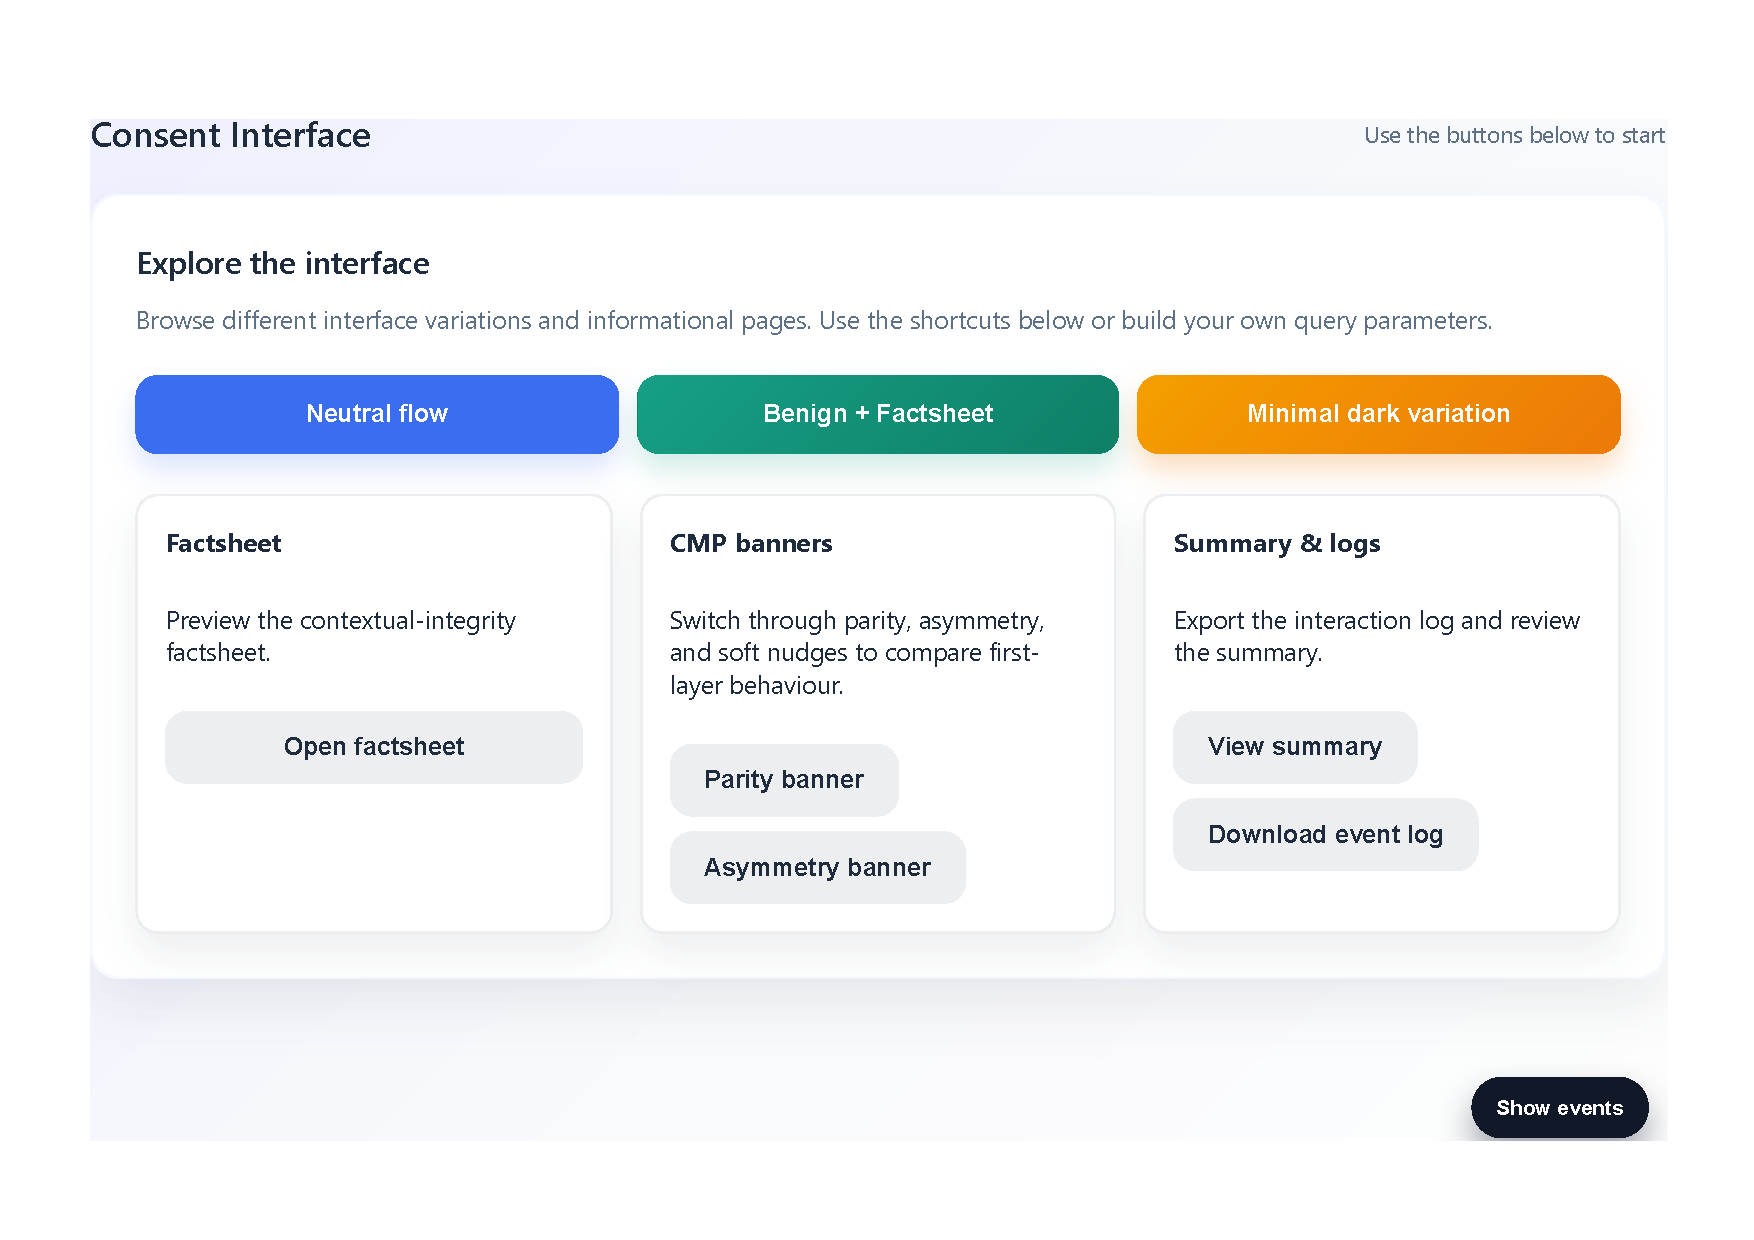
\includegraphics[width=0.85\linewidth]{Figures/consent interface.pdf}
  \caption{Consent interface for the experiment}
  \label{fig:consent}
\end{figure}
\begin{figure}[t]
  \centering
  % Replace with final ABA time‑series plot (vector preferred).
  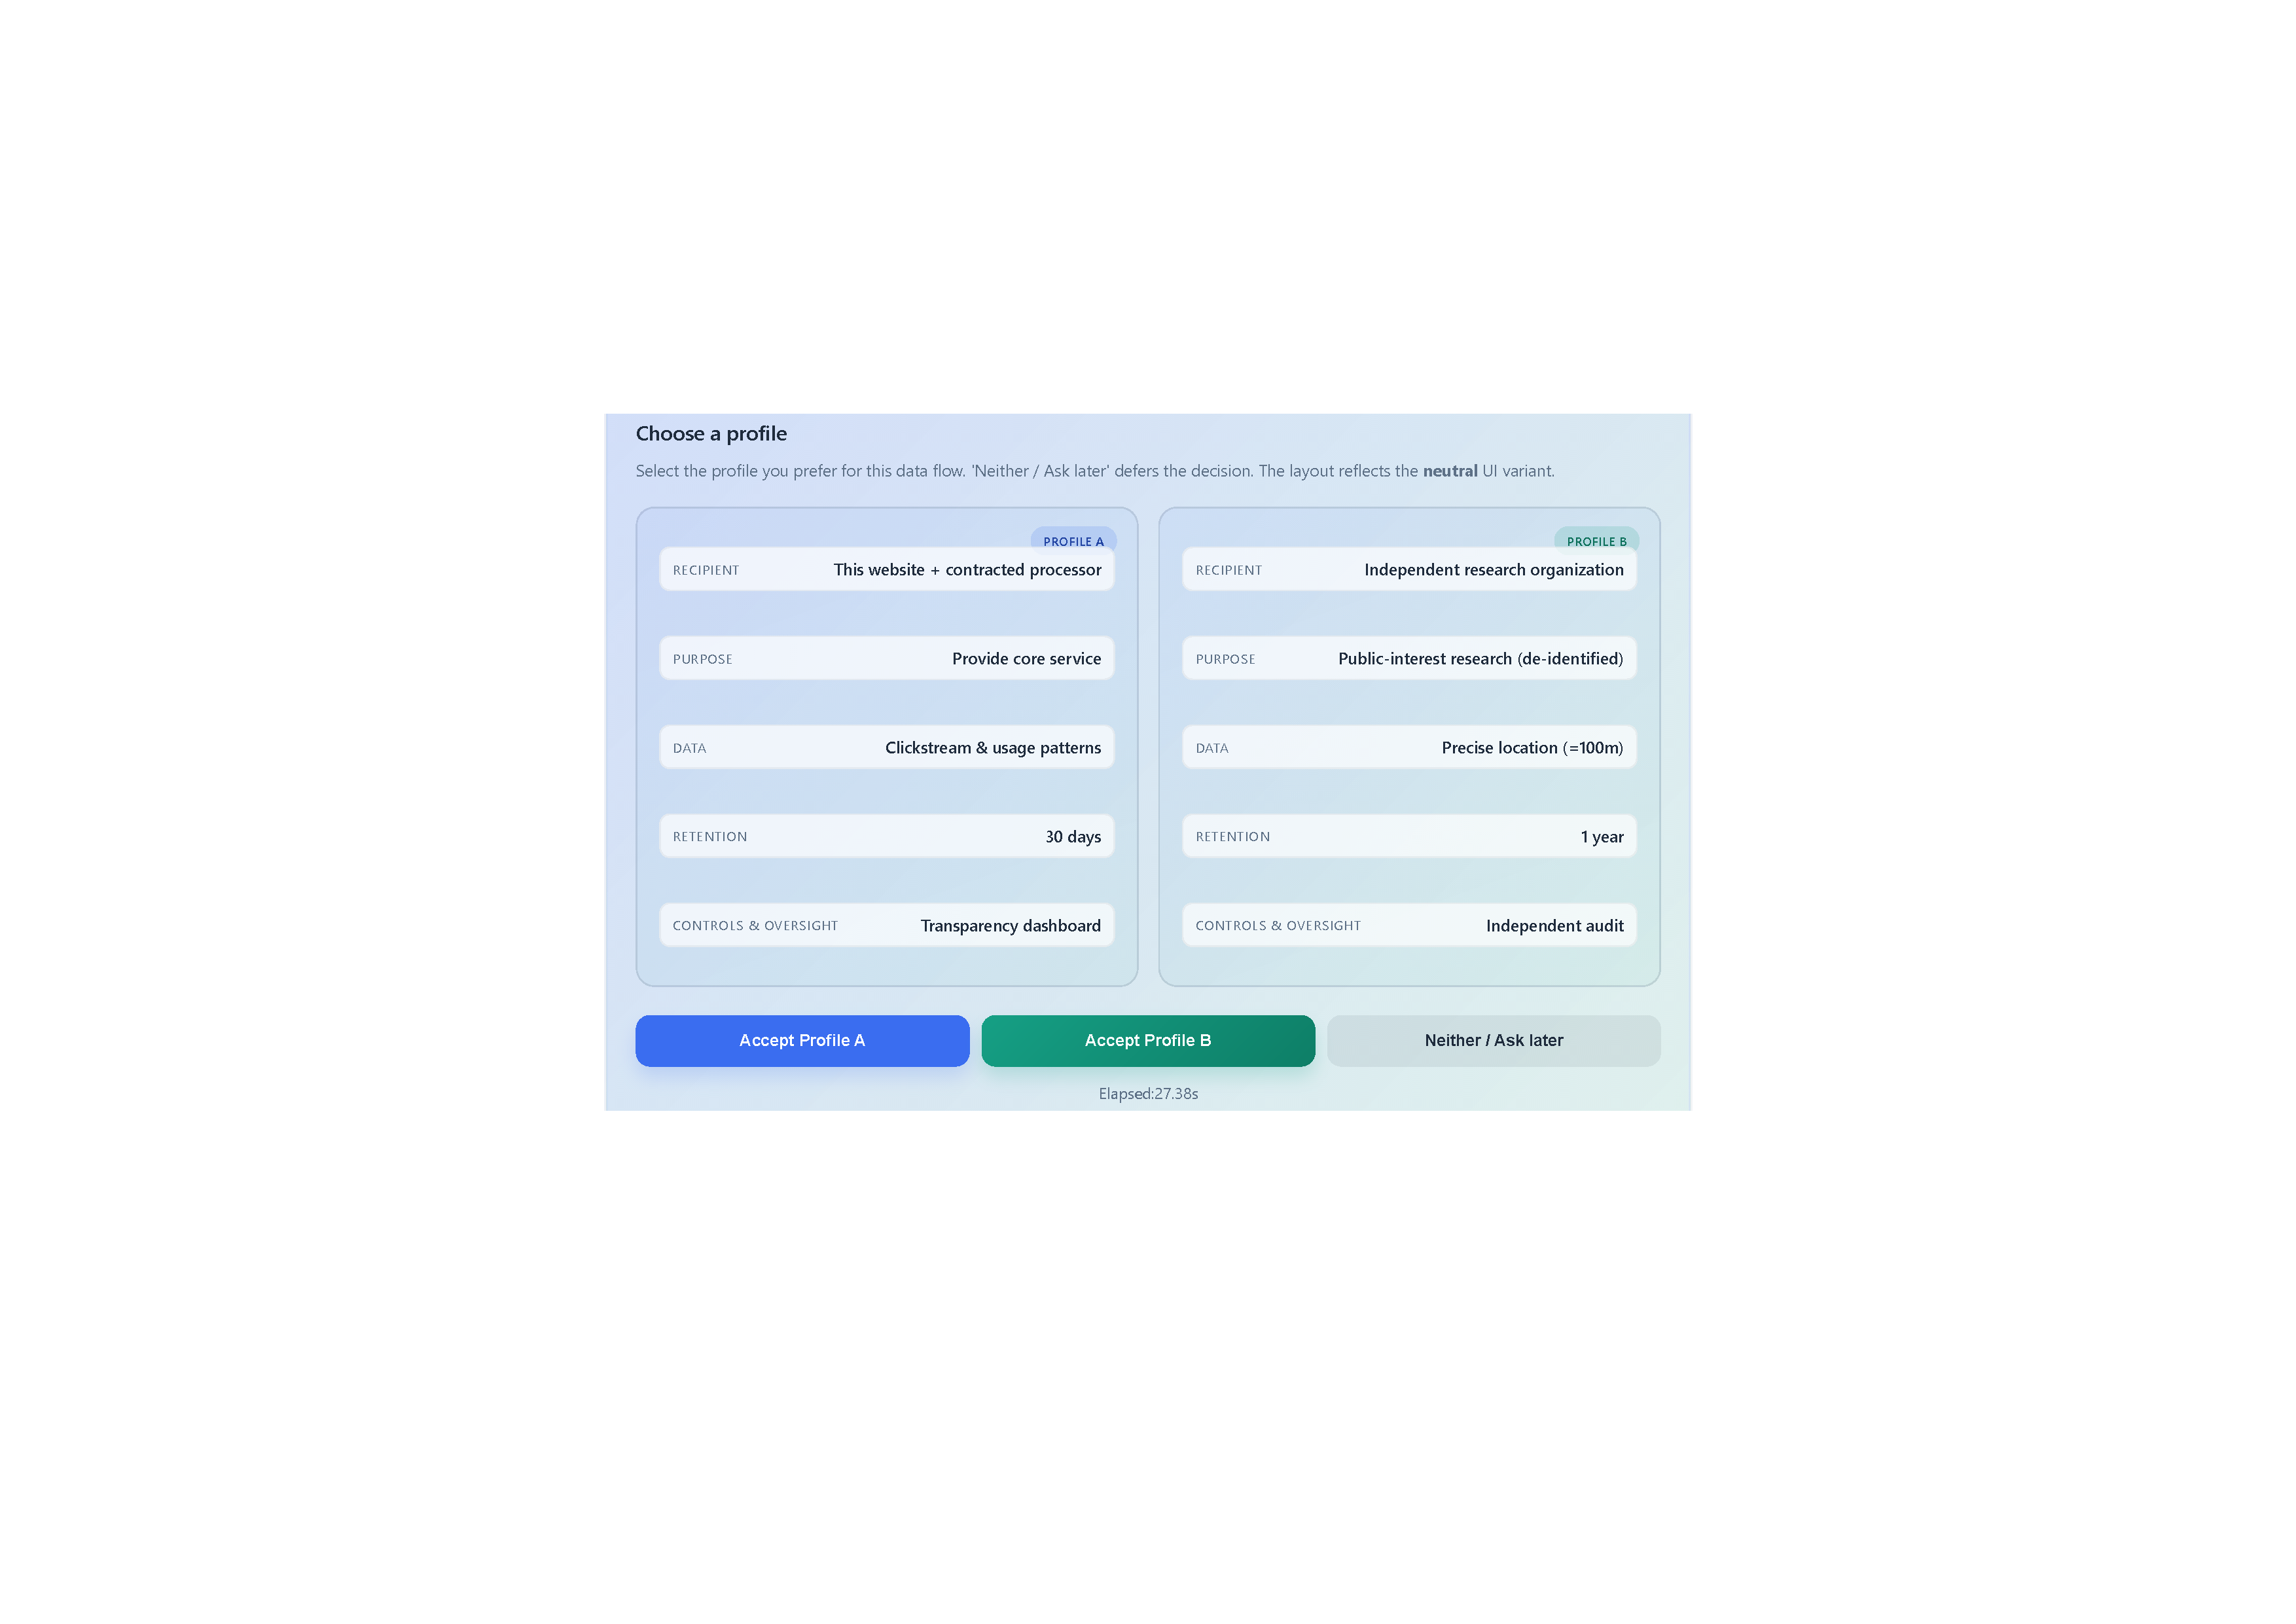
\includegraphics[width=0.85\linewidth]{Figures/profile choose.pdf}
  \caption{Profile selection UI}
  \label{fig:selection}
\end{figure}
\subsection*{CMP-banner mimic (templates)}
We used three layouts: (i) Neutral parity (first-layer ``Accept all'' and ``Reject all'' coequal), (ii) Benign variant (non-persuasive palette/ordering), and (iii) Dark (``Reject all'' behind a ``More options'' click; no pre-ticked boxes). Figure~\ref{fig:ui-appendix} shows redacted screenshots.

\subsection*{Factsheet}
\begin{quote}\small
\textbf{Independent audit \& public report:} An independent organization periodically reviews whether the stated data uses and protections match actual practice and publishes a public report.

\textbf{Delete \& portability (self-serve):} You can view and delete your data at any time and export a machine-readable copy.
\end{quote}

\begin{figure}[t]
  \centering
   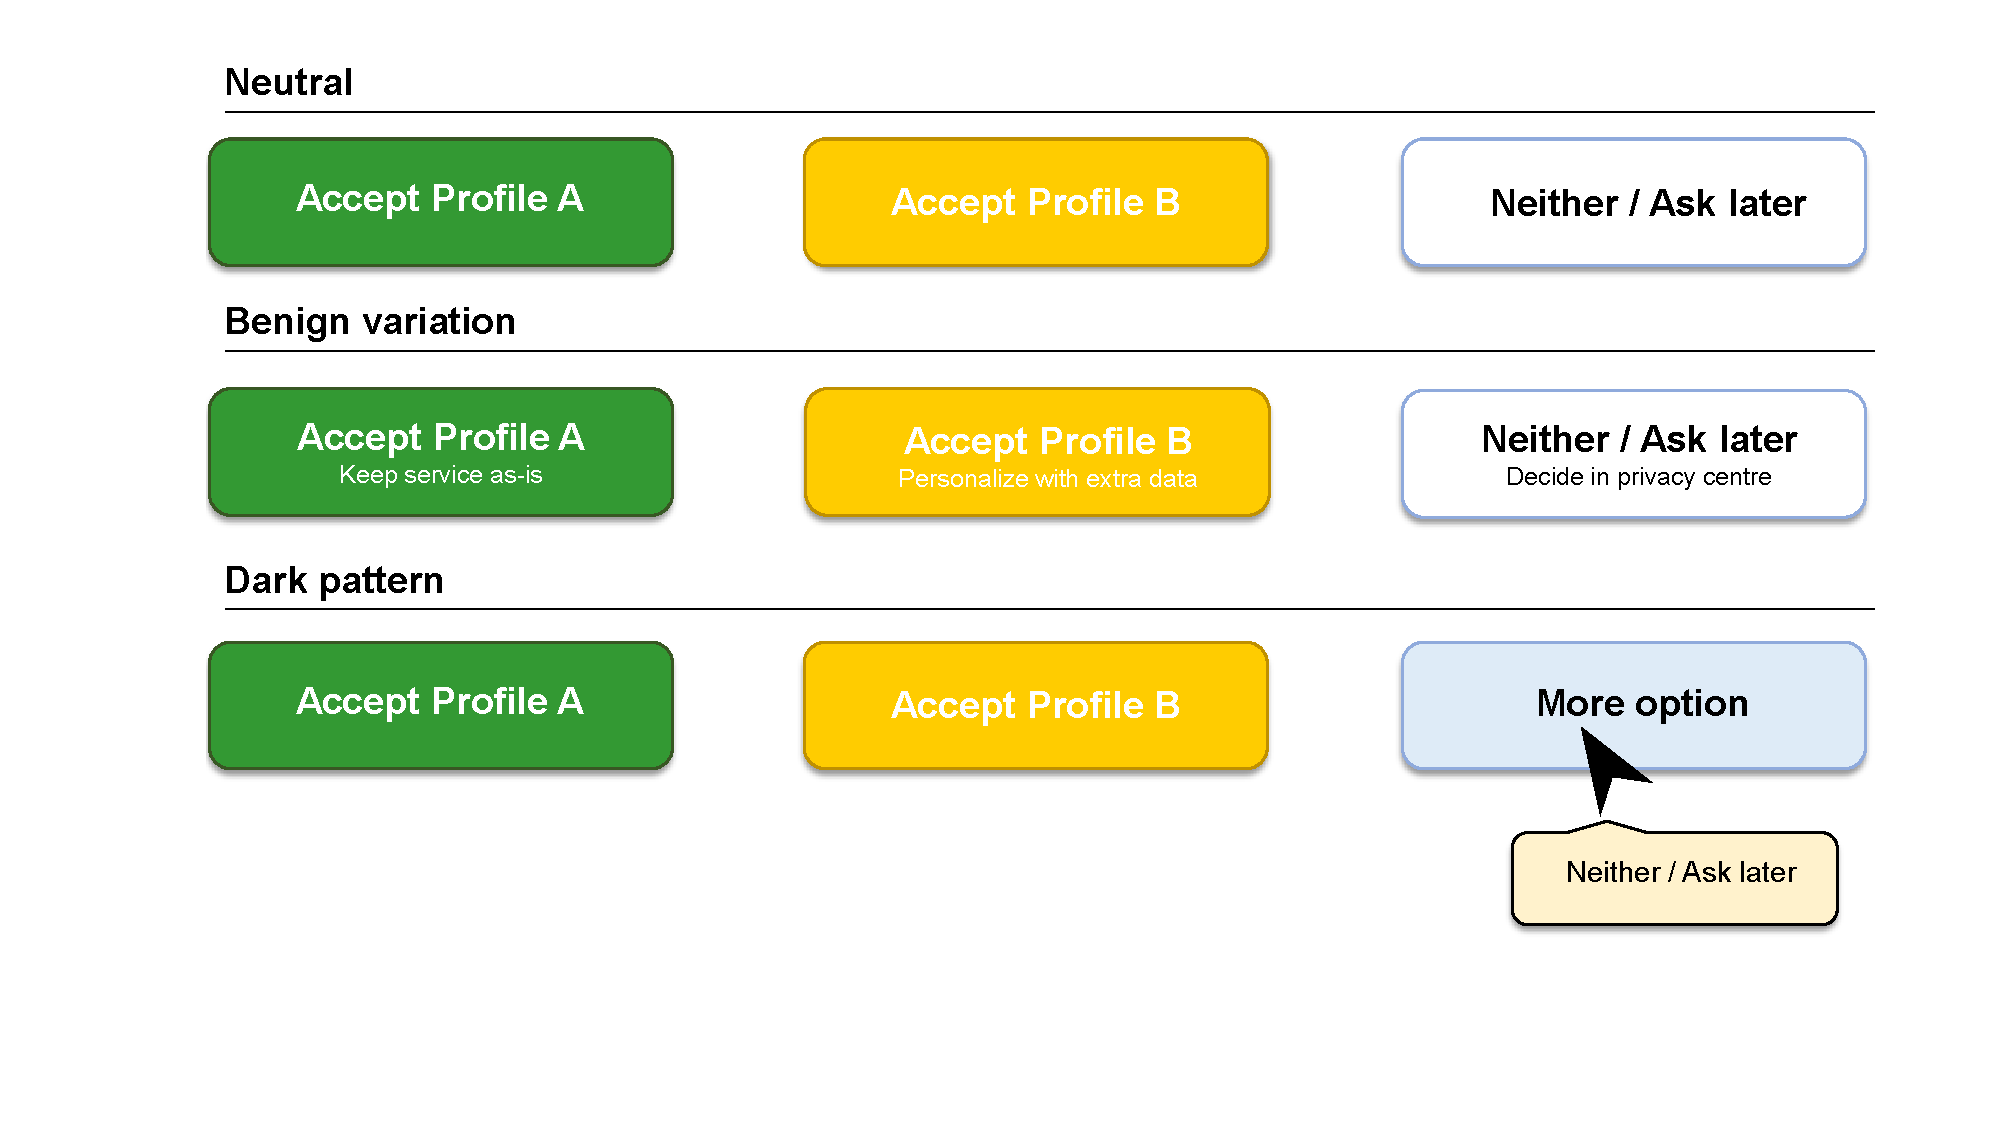
\includegraphics[width=0.85\linewidth]{Figures/ui_variant.pdf}
  \caption{UI variants used in the study}
  \label{fig:ui-appendix}
\end{figure}

\begin{table*}[!htbp]
  \centering
  \resizebox{\linewidth}{!}{%
  \begin{tabular}{l r r r r r}
     & \textbf{Base} & \textbf{Probit} & \textbf{Nested} & \textbf{GMNL} & \textbf{Ordered-Ret} \\
    \hline
    R4 Brokers (AMCE)  & $-0.290$ [$-0.450,-0.120$] & $-0.302$ [$-0.466,-0.135$] & $-0.283$ [$-0.447,-0.117$] & $-0.297$ [$-0.465,-0.132$] & $-0.286$ [$-0.446,-0.118$] \\
    P3 Advertising     & $-0.619$ [$-0.798,-0.458$] & $-0.633$ [$-0.812,-0.470$] & $-0.612$ [$-0.791,-0.451$] & $-0.626$ [$-0.806,-0.464$] & $-0.615$ [$-0.795,-0.454$] \\
    D3 Precise loc.    & $-0.607$ [$-0.803,-0.445$] & $-0.615$ [$-0.812,-0.452$] & $-0.601$ [$-0.797,-0.440$] & $-0.612$ [$-0.808,-0.447$] & $-0.603$ [$-0.799,-0.441$] \\
    D4 Sensitive       & $-0.512$ [$-0.676,-0.352$] & $-0.519$ [$-0.683,-0.359$] & $-0.508$ [$-0.672,-0.348$] & $-0.521$ [$-0.684,-0.360$] & $-0.510$ [$-0.674,-0.350$] \\
    T4 Indefinite      & $-0.548$ [$-0.710,-0.400$] & $-0.556$ [$-0.720,-0.409$] & $-0.541$ [$-0.704,-0.395$] & $-0.553$ [$-0.716,-0.405$] & $-0.536$ [$-0.699,-0.390$] \\
    C3 Delete/port.    & $+0.428$ [$+0.284,+0.592$] & $+0.437$ [$+0.293,+0.601$] & $+0.420$ [$+0.276,+0.584$] & $+0.432$ [$+0.288,+0.596$] & $+0.424$ [$+0.280,+0.588$] \\
    C4 Audit           & $+0.324$ [$+0.212,+0.436$] & $+0.329$ [$+0.217,+0.441$] & $+0.319$ [$+0.207,+0.431$] & $+0.327$ [$+0.215,+0.439$] & $+0.321$ [$+0.209,+0.433$] \\
    \addlinespace
    $\lambda_{\text{Dark}}$ & $0.91$ [$0.84,0.99$] & $0.92$ [$0.85,1.00$] & $0.90$ [$0.83,0.98$] & $0.92$ [$0.85,1.00$] & $0.91$ [$0.84,0.99$] \\
    $\delta_{\text{Dark}}$  & $-0.08$ [$-0.13,-0.03$] & $-0.09$ [$-0.14,-0.04$] & $-0.08$ [$-0.13,-0.03$] & $-0.10$ [$-0.15,-0.05$] & $-0.08$ [$-0.13,-0.03$] \\
    \addlinespace
    S3 $\Delta$\% (Dark--Neutral) & $+7.0$ [$+4.8,+9.4$] & $+7.3$ [$+5.0,+9.7$] & $+6.6$ [$+4.5,+8.9$] & $+7.2$ [$+5.0,+9.6$] & $+6.8$ [$+4.7,+9.1$] \\
  \end{tabular}
  }
  \caption{Robustness of core estimands across model variants (posterior mean [95\% HDI]).}
  \label{tab:robustness}
\end{table*}

\section{Local Probability Mapping in 3-Alternative MNL}
\label{app:probmap}
Let $P(A)=\frac{e^{V_A}}{e^{V_A}+e^{V_B}+e^{V_N}}$, $P(B)$ analogously, and $P(N)$ for Neither. Acceptance $P_{\mathrm{acc}}=P(A)+P(B)$. In MNL,
$\frac{\partial P(j)}{\partial V(i)}=P(j)\big[\mathbb{1}\{i=j\}-P(i)\big]$.
A small utility bump $\Delta u$ applied only to $A$ gives
\[
\frac{\partial P_{\mathrm{acc}}}{\partial V_A}
= \frac{\partial P(A)}{\partial V_A} + \frac{\partial P(B)}{\partial V_A}
= P(A)\big(1-P(A)\big) - P(A)P(B)
= P(A)P(N).
\]
If the same $\Delta u$ is applied to \emph{both} acceptable profiles, then
$\frac{\partial P_{\mathrm{acc}}}{\partial V_A} + \frac{\partial P_{\mathrm{acc}}}{\partial V_B}
= P(N)\big(P(A)+P(B)\big) = P_{\mathrm{acc}}\big(1-P_{\mathrm{acc}}\big).$
In the paper we report full scenario-level posterior predictions; the local derivatives here are provided for intuition only.
\section{Model Parameterization}
\label{app:model_detail}
Let $x\in\mathbb{R}^K$ denote effects-coded attributes and levels. Participant $i$ in UI arm $g(i)\in\{\text{Neutral},\text{Benign},\text{Dark}\}$ chooses alternative $j\in\{A,B,N\}$ in trial $t$ with utility
\begin{equation}\label{eq:hetMNL}
\begin{aligned}
U_{ijt}
&= \lambda_{g(i)}\Big(\beta_i^\top x_{jt} + \alpha_i\,\mathbb{1}[j=N]\Big)
\;+\; \delta_{g(i)}\,\mathbb{1}[j=N]
\;+\; \varepsilon_{ijt},\\[2pt]
&\varepsilon_{ijt}\;\;\text{i.i.d.\ Type-I Extreme Value (Gumbel)}.
\end{aligned}
\end{equation}
Here, $\lambda_{g}$ is an arm-specific scale (Neutral fixed to~$1$); $\beta_i$ are individual utilities; $\alpha_i$ is the participant-specific Neither alternative-specific constant (ASC); and $\delta_g$ is an arm-level incremental penalty on Neither that sits outside the scale term. Individual tastes share a common group mean across arms: $\beta_i\sim \mathcal{N}(\mu,\Sigma)$ irrespective of $g(i)$. We estimate arm-specific scales $\lambda_g$ (with $\lambda_{\text{Neutral}}{=}1$) and an arm-level opt-out penalty $\delta_g$ (with $\delta_{\text{Neutral}}{=}0$), while keeping $\mu$ common.

\section{Statistical Analysis}
\label{subsec:analysis}

We estimated the heteroskedastic HB--MNL in Eq.~\eqref{eq:hetMNL} with $\lambda_{\text{Neutral}}{=}1$ and $\delta_{\text{Neutral}}{=}0$ as identification constraints. Individual utilities follow a common hierarchical prior across UI arms: $\beta_i \sim \mathcal{N}(\mu,\Sigma)$, i.e., \emph{the group mean $\mu$ is shared across arms}. We place weakly informative priors on $\mu$ and $\Sigma$, a weakly informative prior on the Neither ASC $\alpha_i$, and weakly informative priors on $\delta_g$ and $\log\lambda_g$ for $g\in\{\text{Benign},\text{Dark}\}$. CI-motivated interactions receive zero-centered Normal priors with a half-Normal prior on their group standard deviations for shrinkage. We focus inference on AMCEs (pooled), arm-level scale ratios and opt-out penalties, and \emph{scenario-level} acceptance differences.

We reported AMCEs with 95\% highest-density intervals; \emph{no} cross-arm coefficient contrasts are used for inference. Instead, we report (i) the arm-level Neither penalty $\delta_g$ and (ii) \emph{scenario-level} acceptance differences (percentage points) for canonical profiles and CMP-weighted profiles. 

We evaluated hold-out choice accuracy and reliability curves for predictive performance and calibration, and used posterior predictive checks for choice shares including Neither.

On repeated tasks after seven days we computed ICC(2,1) for blockwise utility summaries (Recipient, Purpose, Data, Retention, Controls), the Neither constant, and predicted acceptance. 

We modeled path length to Neither and time to Neither with arm indicators and device class as a covariate. We analyzed perceived friction and first-layer decline recall, and used a symmetric-friction control in the CMP mimic banners to test selective opt-out friction.

We trained Bayesian Rule Lists to approximate HB predictions on hold-outs and reported AUC, accuracy, and median rule length. We clustered scale-normalized utilities via a finite latent-class mixture (classes selected by WAIC), assessed class stability by bootstrap adjusted Rand index and split-half normalized mutual information, and used a greedy expected-information-gain routine to select 3–5 diagnostic questions for cold-start placement, validated on Session~2 and the banner mimic block.

We performed sensitivity analyses without altering the primary estimands: a GMNL extension with individual scale layered on arm scale~\citep{Fiebig2010GMNL}; a monotone random-walk prior for ordered retention; an alternative multinomial probit link and a nested treatment of Neither; attribute non-attendance diagnostics with re-estimation excluding flagged attributes; and profile reweighting under a CMP-weighted distribution from the banner mimic block.

\paragraph{Auxiliary taste-shift model (for Table~\ref{tab:ui_contrasts_appendix}).}
As a sensitivity check on the taste-invariance assumption, we estimated an auxiliary model in which the group mean $\mu$ is allowed to vary by UI arm: $\beta_i \sim \mathcal{N}(\mu_{g(i)},\Sigma)$, with arm-specific means $\mu_g$ sharing a hierarchical shrinkage prior $\mu_g \sim \mathcal{N}(\bar{\mu}, \tau^2 I)$ centered on a global mean $\bar{\mu}$; $\tau \sim \mathrm{Half\text{-}Normal}(0.1)$, encoding a prior expectation of small inter-arm taste differences. Only group means vary by arm; $\Sigma$, $\lambda_g$, and $\delta_g$ retain the same structure as the primary model. Table~\ref{tab:ui_contrasts_appendix} reports two contrasts: ``raw'' differences $\mu_g - \mu_{\text{Neutral}}$ (averaged across coefficients) and ``scale-normalized'' differences $(\mu_g - \mu_{\text{Neutral}})/\lambda_g$, which adjust for arm-specific error variance. These are provided as \emph{diagnostics only}: because arm-level means and scale are partially confounded in logit models, the primary paper reports UI effects exclusively via $\delta_g$ and scenario-level acceptance (Tables~\ref{tab:manip}--\ref{tab:scenarios}). The auxiliary results confirm that Benign--Neutral taste shifts are negligible (HDIs include zero) while the Dark arm shows shifts that are difficult to separate from its lower scale.


\section{Additional Results and Robustness}

\begin{table}[!h]
  \centering
  \begin{tabular}{l l r r r r}
    \textbf{Session} & \textbf{Arm} & \textbf{Path mean} & \textbf{Path SD} & \textbf{Time mean (ms)} & \textbf{Time SD} \\
    \hline
    1 & Neutral & 1.045 & 0.056 & 1651.6 & 231.8 \\
    1 & Benign  & 1.066 & 0.065 & 1655.7 & 224.5 \\
    1 & Dark    & \textbf{2.055} & 0.120 & \textbf{2936.3} & 248.9 \\
    \addlinespace
    2 & Neutral & 1.049 & 0.060 & 1641.3 & 242.1 \\
    2 & Benign  & 1.072 & 0.072 & 1690.2 & 237.5 \\
    2 & Dark    & \textbf{2.041} & 0.125 & \textbf{2958.7} & 261.2 \\
  \end{tabular}
  \caption{Manipulation checks (path length and time to \emph{Neither}) by session and UI arm. Values are means with SD in parentheses. The Dark arm requires roughly double the clicks and time, with minimal change between sessions ($n_{\text{S1}}{=}168$; $n_{\text{S2}}{=}120$).}
  \label{tab:manip_session}
\end{table}


\begin{table}[!h]
  \centering
  \begin{tabular}{l l r r r r}
    \textbf{Session} & \textbf{Arm} & \textbf{Friction mean} & \textbf{Friction SD} & \textbf{Recall mean} & \textbf{Recall SD} \\
    \hline
    1 & Neutral & 2.403 & 0.178 & 0.876 & 0.053 \\
    1 & Benign  & 2.436 & 0.218 & 0.859 & 0.059 \\
    1 & Dark    & \textbf{3.001} & 0.241 & \textbf{0.392} & 0.057 \\
    \addlinespace
    2 & Neutral & 2.417 & 0.186 & 0.871 & 0.056 \\
    2 & Benign  & 2.452 & 0.223 & 0.864 & 0.062 \\
    2 & Dark    & \textbf{2.985} & 0.255 & \textbf{0.404} & 0.064 \\
  \end{tabular}
  \caption{Perceived friction (1--7 scale) and first-layer decline recall (proportion correctly recalling that refusal was available on the first screen) by session and UI arm. The Dark arm shows elevated friction and sharply reduced recall, consistent with the gating manipulation.}
  \label{tab:manip_session_2}
\end{table}


\begin{table}[!h]
  \centering
  \begin{tabular}{l r}
    Observed share A & 0.407 \\
    Predicted share A & 0.405\ [0.397,\ 0.413] \\
    \addlinespace
    Observed share B & 0.404 \\
    Predicted share B & 0.404\ [0.396,\ 0.412] \\
    \addlinespace
    Observed share Neither & 0.189 \\
    Predicted share Neither & 0.191\ [0.184,\ 0.198] \\
    \addlinespace
    Multiclass Brier score & 0.192 \\
    Expected calibration error (ECE) & 0.023 \\
    Maximum calibration error (MCE) & 0.061 \\
    Log loss (cross-entropy) & 1.014 \\
  \end{tabular}
  \caption{Posterior predictive checks (Session~1). Predicted class shares (mean [95\% HDI]) closely match observed. Multiclass Brier and ECE indicate good calibration.}
  \label{tab:ppc_stats}
\end{table}


\begin{table}[h]
  \centering
  \resizebox{\linewidth}{!}{%
  \begin{tabular}{@{} l l r @{}}
    \textbf{Interaction} & \textbf{Label} & \textbf{Estimate [95\% HDI]} \\
    \hline
    Recipient (R4 Brokers) $\times$ Retention (T4 Indefinite) & R4$\times$T4 & $-0.323\ [-0.470,\ -0.180]$ \\
    Purpose (P3 Advertising) $\times$ Data (D4 Sensitive)      & P3$\times$D4 & $-1.033\ [-1.250,\ -0.820]$ \\
    Purpose (P2 Personalization) $\times$ Data (D4 Sensitive)  & P2$\times$D4 & $-0.047\ [-0.180,\ +0.090]$ \\
    Recipient (R4 Brokers) $\times$ Controls (C3 Delete)       & R4$\times$C3 & $-0.367\ [-0.550,\ -0.190]$ \\
    Recipient (R4 Brokers) $\times$ Controls (C4 Audit)        & R4$\times$C4 & $+0.697\ [+0.520,\ +0.880]$ \\
  \end{tabular}
  }
  \caption{Prespecified CI-motivated two-way interactions (posterior mean [95\% HDI]). P3$\times$D4 shows the strongest compounding disutility; R4$\times$C4 shows that Independent audit substantially mitigates broker-specific disutility. All estimates use hierarchical shrinkage priors.}
  \label{tab:interactions}
\end{table}
\begin{table}[h]
  \centering
  \begin{tabular}{l r r}
    \textbf{Arm} & \textbf{Scenario acceptance} & \textbf{CMP-weighted acceptance} \\
    \hline
    Neutral & 0.606 & 0.618 \\
    Benign  & 0.597 & 0.602 \\
    Dark    & 0.622 & 0.663 \\
  \end{tabular}
  \caption{Scenario-level acceptance under the experimental design distribution vs.\ CMP-weighted profile distribution (posterior means). Differences are small, indicating that inferences are not sensitive to the profile distribution.}
  \label{tab:profilesens_table}
\end{table}

\begin{table}[h]
  \centering
  \begin{tabular}{l r r r r}
    \textbf{Factor} & \textbf{L1} & \textbf{L2} & \textbf{L3} & \textbf{L4} \\
    \hline
    Recipient (R1,R2,R3,R4) & 0.45 & 0.10 & 0.07 & 0.38 \\
    Purpose (P1,P2,P3,P4)   & 0.29 & 0.36 & 0.35 & 0.00 \\
    Data (D1,D2,D3,D4)      & 0.28 & 0.34 & 0.22 & 0.16 \\
    Retention (T1,T2,T3,T4) & 0.16 & 0.27 & 0.33 & 0.24 \\
    Controls (C1,C2,C3,C4)  & 0.48 & 0.22 & 0.18 & 0.12 \\
  \end{tabular}
  \caption{CMP-banner mimic profile frequencies used for reweighting. L1--L4 correspond to levels 1--4 within each factor (see Table~\ref{tab:attributes}). The CMP distribution is skewed toward first-party recipients (R1) and no-controls (C1), reflecting typical banner configurations.}
  \label{tab:cmpdist}
\end{table}


\begin{table}[h]
  \centering
  \begin{tabular}{l r r}
    \textbf{Arm} & \textbf{Accept} & \textbf{Reject} \\
    \hline
    Neutral & 0.566 & 0.434 \\
    Benign  & 0.548 & 0.452 \\
    Dark    & \textbf{0.620} & 0.380 \\
  \end{tabular}
  \caption{CMP-banner mimic acceptance and rejection rates by UI arm (means across four one-screen banners). The Dark arm raises acceptance by +5.4 percentage points relative to Neutral, consistent with selective opt-out friction.}
  \label{tab:cmp_accept}
\end{table}

\noindent Participant-level micro-game Neither-propensity aligned with CMP Reject-all (Spearman $\rho=0.49$, $p<10^{-10}$). The alignment remained when conditioning on predicted acceptance of A/B (partial $\rho\approx 0.40$).

\begin{table}[!h]
  \centering
  \begin{tabular}{l l r r r}
    \textbf{Arm} & \textbf{Contrast} & \textbf{Mean} & \textbf{95\% HDI low} & \textbf{95\% HDI high} \\
    \hline
    Benign & Raw              & 0.090 & -0.102 & 0.290 \\
    Benign & Scale-normalized & 0.105 & -0.120 & 0.360 \\
    Dark   & Raw              & \textbf{-0.338} & -0.575 & -0.119 \\
    Dark   & Scale-normalized & \textbf{-0.453} & -0.854 & -0.149 \\
  \end{tabular}
  \caption{Auxiliary sensitivity check: coefficient contrasts from a model that allows arm-specific group means $\mu_g$ (not the primary specification, which shares $\mu$ across arms). The Benign arm shows negligible taste shifts (HDIs include zero), supporting the invariance assumption. The Dark arm shows credible negative shifts that widen after scale normalization; because these coefficients are confounded with scale and friction in this auxiliary model, the primary paper reports UI effects only via $\delta_g$ and scenario-level acceptance (Table~\ref{tab:scenarios}). This table is provided as a diagnostic, not for cross-arm taste inference.}
  \label{tab:ui_contrasts_appendix}
\end{table}

\begin{table}[!h]
  \centering
  \begin{tabular}{l r r}
    \textbf{Attribute} & \textbf{Stated ANA \%} & \textbf{Inferred ANA \%} \\
    \hline
    Recipient & 3.0 & 2.4 \\
    Purpose   & 6.5 & 5.8 \\
    Data type & 5.9 & 5.1 \\
    Retention & 4.1 & 3.7 \\
    Controls  & 4.8 & 4.2 \\
  \end{tabular}
  \caption{Attribute non-attendance (ANA) prevalence: stated (self-reported) and inferred (variance-based diagnostic). All rates are below 7\%, with no attribute showing a reversal between stated and inferred measures. Low ANA supports the interpretability of utility estimates.}
  \label{tab:ana}  
\end{table}

\section{Consolidated Robustness Across Specifications}
Table~\ref{tab:robustness} summarizes core estimands across five specifications: baseline heteroskedastic HB--MNL (this paper), multinomial probit, nested logit with \Neither{} as a separate nest, GMNL (individual scale layered on arm-scale), and an ordered-prior variant for retention.

\end{document}
